%% SKIPPED wegens lonely items \documentclass{ximera}

%
%%% Begin Laad packages
%
\makeatletter
\@ifclassloaded{xourse}{%
    \typeout{Start loading preamble.tex (in a XOURSE)}%
    \def\isXourse{true}   % automatically defined; pre 112022 it had to be set 'manually' in a xourse
}{%
    \typeout{Start loading preamble.tex (NOT in a XOURSE)}%
}
\makeatother

\pgfplotsset{compat=1.16}

\usepackage{currfile}

% 201908/202301: PAS OP: babel en doclicense lijken problemen te veroorzaken in .jax bestand
% (wegens syntax error met toegevoegde \newcommands ...)
\pdfOnly{
    \usepackage[hyperxmp=false,type={CC},modifier={by-nc-sa},version={4.0}]{doclicense}
    \usepackage[dutch]{babel}
}


\usepackage[utf8]{inputenc}
\usepackage{morewrites}   % nav zomercursus (answer...?)
\usepackage{multirow}
\usepackage{multicol}
\usepackage{tikzsymbols}
\usepackage{tikz-3dplot}
\usepackage{ifthen}
%\usepackage{animate} BREAKS HTML STRUCTURE USED BY XIMERA
\usepackage{relsize}

\usepackage{eurosym}    % \euro  (€ werkt niet in xake ...?)
\usepackage{wrapfig}

\usepackage{cancel}

\usepackage{tabularx}
% Nuttig als ook interactieve beamer slides worden voorzien:
\providecommand{\p}{} % default nothing ; potentially usefull for slides: redefine as \pause
%providecommand{\p}{\pause}

\usepackage{caption} % captionof
%\usepackage{pdflscape}    % landscape environment

% Met "\newcommand\showtodonotes{}" kan je todonotes tonen (in pdf/online)
% 201908: online werkt het niet (goed)
\providecommand\showtodonotes{disable}
\providecommand\todo[1]{\typeout{TODO #1}}
%\usepackage[\showtodonotes]{todonotes}
%\usepackage{todonotes}

%
% Poging tot aanpassen layout
%
\usepackage{tcolorbox}
\tcbuselibrary{theorems}

%%% Einde laad packages

%%% Begin Ximera specifieke zaken

% \graphicspath{
% 	{../../}
% 	{../}
% 	{./}
%   	{../../pictures/}
%    	{../pictures/}
%    	{./pictures/}
% 	{./explog/}    % M05 in groeimodellen       
% }

%%% Einde Ximera specifieke zaken

%
% define softer blue/red/green, use KU Leuven base colors for blue (and dark orange for red ?)
%
% todo: rather redefine blue/red/green ...?
%\definecolor{xmblue}{rgb}{0.01, 0.31, 0.59}
%\definecolor{xmred}{rgb}{0.89, 0.02, 0.17}
\definecolor{xmdarkblue}{rgb}{0.122, 0.671, 0.835}   % KU Leuven Blauw
\definecolor{xmblue}{rgb}{0.114, 0.553, 0.69}        % KU Leuven Blauw
\definecolor{xmgreen}{rgb}{0.13, 0.55, 0.13}         % No KULeuven variant for green found ...

\definecolor{xmaccent}{rgb}{0.867, 0.541, 0.18}      % KU Leuven Accent (orange ...)
\definecolor{kuaccent}{rgb}{0.867, 0.541, 0.18}      % KU Leuven Accent (orange ...)

\colorlet{xmred}{xmaccent!50!black}                  % Darker version of KU Leuven Accent

\providecommand{\blue}[1]{{\color{blue}#1}}    
\providecommand{\red}[1]{{\color{red}#1}}

\renewcommand\CancelColor{\color{xmaccent!50!black}}

% werkt in math en text mode om MATH met oranje (of grijze...)  achtergond te tonen (ook \important{\text{blabla}} lijkt te werken)
%\newcommand{\important}[1]{\ensuremath{\colorbox{xmaccent!50!white}{$#1$}}}   % werkt niet in Mathjax
%\newcommand{\important}[1]{\ensuremath{\colorbox{lightgray}{$#1$}}}
%\newcommand{\important}[1]{\ensuremath{\colorbox{orange}{$#1$}}}   % TODO: kleur aanpassen voor mathjax; wordt overschreven infra!
\newcommand{\important}[1]{\ensuremath{\fcolorbox{black}{white}{$#1$}}}


% Uitzonderlijk kan met \pdfnl in de PDF een newline worden geforceerd, die online niet nodig/nuttig is omdat daar de regellengte hoe dan ook niet gekend is.
\ifdefined\HCode%
\providecommand{\pdfnl}{}%
\else%
\providecommand{\pdfnl}{%
  \\%
}%
\fi

% Uitzonderlijk kan met \handoutnl in de handout-PDF een newline worden geforceerd, die noch online noch in de PDF-met-antwoorden nuttig is.
\ifdefined\HCode
\providecommand{\handoutnl}{}
\else
\providecommand{\handoutnl}{%
\ifhandout%
  \nl%
\fi%
}
\fi



% \cellcolor IGNORED by tex4ht ?
% \begin{center} seems not to wordk
    % (missing margin-left: auto;   on tabular-inside-center ???)
%\newcommand{\importantcell}[1]{\ensuremath{\cellcolor{lightgray}#1}}  %  in tabular; usablility to be checked
\providecommand{\importantcell}[1]{\ensuremath{#1}}     % no mathjax2 support for colloring array cells

\pdfOnly{
  \renewcommand{\important}[1]{\ensuremath{\colorbox{kuaccent!50!white}{$#1$}}}
  \renewcommand{\importantcell}[1]{\ensuremath{\cellcolor{kuaccent!40!white}#1}}   
}

%%% Tikz styles


\pgfplotsset{compat=1.16}

\usetikzlibrary{trees,positioning,arrows,fit,shapes,math,calc,decorations.markings,through,intersections,patterns,matrix}

\usetikzlibrary{decorations.pathreplacing,backgrounds}    % 5/2023: from experimental


\usetikzlibrary{angles,quotes}

\usepgfplotslibrary{fillbetween} % bepaalde_integraal
\usepgfplotslibrary{polar}    % oa voor poolcoordinaten.tex

\pgfplotsset{ownstyle/.style={axis lines = center, axis equal image, xlabel = $x$, ylabel = $y$, enlargelimits}} 

\pgfplotsset{
	plot/.style={no marks,samples=50}
}

\newcommand{\xmPlotsColor}{
	\pgfplotsset{
		plot1/.style={darkgray,no marks,samples=100},
		plot2/.style={lightgray,no marks,samples=100},
		plotresult/.style={blue,no marks,samples=100},
		plotblue/.style={blue,no marks,samples=100},
		plotred/.style={red,no marks,samples=100},
		plotgreen/.style={green,no marks,samples=100},
		plotpurple/.style={purple,no marks,samples=100}
	}
}
\newcommand{\xmPlotsBlackWhite}{
	\pgfplotsset{
		plot1/.style={black,loosely dashed,no marks,samples=100},
		plot2/.style={black,loosely dotted,no marks,samples=100},
		plotresult/.style={black,no marks,samples=100},
		plotblue/.style={black,no marks,samples=100},
		plotred/.style={black,dotted,no marks,samples=100},
		plotgreen/.style={black,dashed,no marks,samples=100},
		plotpurple/.style={black,dashdotted,no marks,samples=100}
	}
}


\newcommand{\xmPlotsColorAndStyle}{
	\pgfplotsset{
		plot1/.style={darkgray,no marks,samples=100},
		plot2/.style={lightgray,no marks,samples=100},
		plotresult/.style={blue,no marks,samples=100},
		plotblue/.style={xmblue,no marks,samples=100},
		plotred/.style={xmred,dashed,thick,no marks,samples=100},
		plotgreen/.style={xmgreen,dotted,very thick,no marks,samples=100},
		plotpurple/.style={purple,no marks,samples=100}
	}
}


%\iftikzexport
\xmPlotsColorAndStyle
%\else
%\xmPlotsBlackWhite
%\fi
%%%


%
% Om venndiagrammen te arceren ...
%
\makeatletter
\pgfdeclarepatternformonly[\hatchdistance,\hatchthickness]{north east hatch}% name
{\pgfqpoint{-1pt}{-1pt}}% below left
{\pgfqpoint{\hatchdistance}{\hatchdistance}}% above right
{\pgfpoint{\hatchdistance-1pt}{\hatchdistance-1pt}}%
{
	\pgfsetcolor{\tikz@pattern@color}
	\pgfsetlinewidth{\hatchthickness}
	\pgfpathmoveto{\pgfqpoint{0pt}{0pt}}
	\pgfpathlineto{\pgfqpoint{\hatchdistance}{\hatchdistance}}
	\pgfusepath{stroke}
}
\pgfdeclarepatternformonly[\hatchdistance,\hatchthickness]{north west hatch}% name
{\pgfqpoint{-\hatchthickness}{-\hatchthickness}}% below left
{\pgfqpoint{\hatchdistance+\hatchthickness}{\hatchdistance+\hatchthickness}}% above right
{\pgfpoint{\hatchdistance}{\hatchdistance}}%
{
	\pgfsetcolor{\tikz@pattern@color}
	\pgfsetlinewidth{\hatchthickness}
	\pgfpathmoveto{\pgfqpoint{\hatchdistance+\hatchthickness}{-\hatchthickness}}
	\pgfpathlineto{\pgfqpoint{-\hatchthickness}{\hatchdistance+\hatchthickness}}
	\pgfusepath{stroke}
}
%\makeatother

\tikzset{
    hatch distance/.store in=\hatchdistance,
    hatch distance=10pt,
    hatch thickness/.store in=\hatchthickness,
   	hatch thickness=2pt
}

\colorlet{circle edge}{black}
\colorlet{circle area}{blue!20}


\tikzset{
    filled/.style={fill=green!30, draw=circle edge, thick},
    arceerl/.style={pattern=north east hatch, pattern color=blue!50, draw=circle edge},
    arceerr/.style={pattern=north west hatch, pattern color=yellow!50, draw=circle edge},
    outline/.style={draw=circle edge, thick}
}




%%% Updaten commando's
\def\hoofding #1#2#3{\maketitle}     % OBSOLETE ??

% we willen (bijna) altijd \geqslant ipv \geq ...!
\newcommand{\geqnoslant}{\geq}
\renewcommand{\geq}{\geqslant}
\newcommand{\leqnoslant}{\leq}
\renewcommand{\leq}{\leqslant}

% Todo: (201908) waarom komt er (soms) underlined voor emph ...?
\renewcommand{\emph}[1]{\textit{#1}}

% API commando's

\newcommand{\ds}{\displaystyle}
\newcommand{\ts}{\textstyle}  % tegenhanger van \ds   (Ximera zet PER  DEFAULT \ds!)

% uit Zomercursus-macro's: 
\newcommand{\bron}[1]{\begin{scriptsize} \emph{#1} \end{scriptsize}}     % deprecated ...?


%definities nieuwe commando's - afkortingen veel gebruikte symbolen
\newcommand{\R}{\ensuremath{\mathbb{R}}}
\newcommand{\Rnul}{\ensuremath{\mathbb{R}_0}}
\newcommand{\Reen}{\ensuremath{\mathbb{R}\setminus\{1\}}}
\newcommand{\Rnuleen}{\ensuremath{\mathbb{R}\setminus\{0,1\}}}
\newcommand{\Rplus}{\ensuremath{\mathbb{R}^+}}
\newcommand{\Rmin}{\ensuremath{\mathbb{R}^-}}
\newcommand{\Rnulplus}{\ensuremath{\mathbb{R}_0^+}}
\newcommand{\Rnulmin}{\ensuremath{\mathbb{R}_0^-}}
\newcommand{\Rnuleenplus}{\ensuremath{\mathbb{R}^+\setminus\{0,1\}}}
\newcommand{\N}{\ensuremath{\mathbb{N}}}
\newcommand{\Nnul}{\ensuremath{\mathbb{N}_0}}
\newcommand{\Z}{\ensuremath{\mathbb{Z}}}
\newcommand{\Znul}{\ensuremath{\mathbb{Z}_0}}
\newcommand{\Zplus}{\ensuremath{\mathbb{Z}^+}}
\newcommand{\Zmin}{\ensuremath{\mathbb{Z}^-}}
\newcommand{\Znulplus}{\ensuremath{\mathbb{Z}_0^+}}
\newcommand{\Znulmin}{\ensuremath{\mathbb{Z}_0^-}}
\newcommand{\C}{\ensuremath{\mathbb{C}}}
\newcommand{\Cnul}{\ensuremath{\mathbb{C}_0}}
\newcommand{\Cplus}{\ensuremath{\mathbb{C}^+}}
\newcommand{\Cmin}{\ensuremath{\mathbb{C}^-}}
\newcommand{\Cnulplus}{\ensuremath{\mathbb{C}_0^+}}
\newcommand{\Cnulmin}{\ensuremath{\mathbb{C}_0^-}}
\newcommand{\Q}{\ensuremath{\mathbb{Q}}}
\newcommand{\Qnul}{\ensuremath{\mathbb{Q}_0}}
\newcommand{\Qplus}{\ensuremath{\mathbb{Q}^+}}
\newcommand{\Qmin}{\ensuremath{\mathbb{Q}^-}}
\newcommand{\Qnulplus}{\ensuremath{\mathbb{Q}_0^+}}
\newcommand{\Qnulmin}{\ensuremath{\mathbb{Q}_0^-}}

\newcommand{\perdef}{\overset{\mathrm{def}}{=}}
\newcommand{\pernot}{\overset{\mathrm{notatie}}{=}}
\newcommand\perinderdaad{\overset{!}{=}}     % voorlopig gebruikt in limietenrekenregels
\newcommand\perhaps{\overset{?}{=}}          % voorlopig gebruikt in limietenrekenregels

\newcommand{\degree}{^\circ}


\DeclareMathOperator{\dom}{dom}     % domein
\DeclareMathOperator{\codom}{codom} % codomein
\DeclareMathOperator{\bld}{bld}     % beeld
\DeclareMathOperator{\graf}{graf}   % grafiek
\DeclareMathOperator{\rico}{rico}   % richtingcoëfficient
\DeclareMathOperator{\co}{co}       % coordinaat
\DeclareMathOperator{\gr}{gr}       % graad

\newcommand{\func}[5]{\ensuremath{#1: #2 \rightarrow #3: #4 \mapsto #5}} % Easy to write a function


% Operators
\DeclareMathOperator{\bgsin}{bgsin}
\DeclareMathOperator{\bgcos}{bgcos}
\DeclareMathOperator{\bgtan}{bgtan}
\DeclareMathOperator{\bgcot}{bgcot}
\DeclareMathOperator{\bgsinh}{bgsinh}
\DeclareMathOperator{\bgcosh}{bgcosh}
\DeclareMathOperator{\bgtanh}{bgtanh}
\DeclareMathOperator{\bgcoth}{bgcoth}

% Oude \Bgsin etc deprecated: gebruik \bgsin, en herdefinieer dat als je Bgsin wil!
%\DeclareMathOperator{\cosec}{cosec}    % not used? gebruik \csc en herdefinieer

% operatoren voor differentialen: to be verified; 1/2020: inconsequent gebruik bij afgeleiden/integralen
\renewcommand{\d}{\mathrm{d}}
\newcommand{\dx}{\d x}
\newcommand{\dd}[1]{\frac{\mathrm{d}}{\mathrm{d}#1}}
\newcommand{\ddx}{\dd{x}}

% om in voorbeelden/oefeningen de notatie voor afgeleiden te kunnen kiezen
% Usage: \afg{(2\sin(x))}  (en wordt d/dx, of accent, of D )
% \afg kan evt al gedefinieerd zijn in xmPreamble, of overschreven worden  
\providecommand{\afg}[1]{\frac{\mathrm{d}}{\mathrm{d}x} \left(#1\right) }   % include in relevant exercises ...
% \providecommand{\afg}[1]{\left{#1\right}'}   
%\renewcommand{\afg}[1]{D\left{#1\right}}

%
% \xmxxx commands: Extra KU Leuven functionaliteit van, boven of naast Ximera
%   ( Conventie 8/2019: xm+nederlandse omschrijving, maar is niet consequent gevolgd, en misschien ook niet erg handig !)
%
% (Met een minimale ximera.cls en preamble.tex zou een bruikbare .pdf moeten kunnen worden gemaakt van eender welke ximera)
%
% Usage: \xmtitle[Mijn korte abstract]{Mijn titel}{Mijn abstract}
% Eerste command na \begin{document}:
%  -> definieert de \title
%  -> definieert de abstract
%  -> doet \maketitle ( dus: print de hoofding als 'chapter' of 'sectie')
% Optionele parameter geeft eenn kort abstract (die met de globale setting \xmshortabstract{} al dan niet kan worden geprint.
% De optionele korte abstract kan worden gebruikt voor pseudo-grappige abtsarts, dus dus globaal al dan niet kunnen worden gebuikt...
% Globale settings:
%  de (optionele) 'korte abstract' wordt enkele getoond als \xmshortabstract is gezet
\providecommand\xmshortabstract{} % default: print (only!) short abstract if present
\providecommand\theabstract{} % otherwise complaint Undefined control sequence.  <recently read> \theabstract  ????
\newcommand{\xmtitle}[3][]{
	\title{#2}
	% \begin{abstract}
	% 			\ifdefined\xmshortabstract
	% 			\ifstrempty{#1}{%
	% 						#3
	% 			}{%
	% 						#1
	% 			}%
	% 			\else
	% 			#3
	% 			\fi
	% \end{abstract}
	\maketitle
}

% 
% Kleine grapjes: moeten zonder verder gevolg kunnen worden verwijderd
%
%\newcommand{\xmopje}[1]{{\small#1{\reversemarginpar\marginpar{\Smiley}}}}   % probleem in floats!!
\newtoggle{showxmopje}
\toggletrue{showxmopje}

\newcommand{\xmopje}[1]{%
   \iftoggle{showxmopje}{#1}{}%
}


% -> geef een abstracte-formule-met-rechts-een-concreet-voorbeeld
% VB:  \formulevb{a^2+b^2=c^2}{3^2+4^2=5^2}
%
\ifdefined\HCode
\NewEnviron{xmdiv}[1]{\HCode{\Hnewline<div class="#1">\Hnewline}\BODY{\HCode{\Hnewline</div>\Hnewline}}}
\else
\NewEnviron{xmdiv}[1]{\BODY}
\fi

\providecommand{\formulevb}[2]{
	{\centering

    \begin{xmdiv}{xmformulevb}    % zie css voor online layout !!!
	\begin{tabular}{lcl}
		\important{#1}
		&  &
		 {$#2$}
		\end{tabular}
	\end{xmdiv}
	}
}

\ifdefined\HCode
\providecommand{\xmcolorbox}[2]{
	\HCode{\Hnewline<div class="xmcolorbox">\Hnewline}#2\HCode{\Hnewline</div>\Hnewline}
}
\else
\providecommand{\xmcolorbox}[2]{
  \cellcolor{#1}#2
}
\fi


\ifdefined\HCode
\providecommand{\xmopmerking}[1]{
 \HCode{\Hnewline<div class="xmopmerking">\Hnewline}#1\HCode{\Hnewline</div>\Hnewline}
}
\else
\providecommand{\xmopmerking}[1]{
	{\footnotesize #1}
}
\fi
% \providecommand{\voorbeeld}[1]{
% 	\colorbox{blue!10}{$#1$}
% }



% Hernoem Proof naar Bewijs, nodig voor HTML versie
\renewcommand*{\proofname}{Bewijs}

% Om opgave van oefening (wordt niet geprint bij oplossingenblad)
% (to be tested test)
\NewEnviron{statement}{\BODY}

% Environment 'oplossing' en 'uitkomst'
% voor resp. volledige 'uitwerking' dan wel 'enkel eindresultaat'
% geimplementeerd via feedback, omdat er in de ximera-server adhoc feedback-code is toegevoegd
%% Niet tonen indien handout
%% Te gebruiken om volledige oplossingen/uitwerkingen van oefeningen te tonen
%% \begin{oplossing}        De optelling is commutatief \end{oplossing}  : verschijnt online enkel 'op vraag'
%% \begin{oplossing}[toon]  De optelling is commutatief \end{oplossing}  : verschijnt steeds onmiddellijk online (bv te gebruiken bij voorbeelden) 

\ifhandout%
    \NewEnviron{oplossing}[1][onzichtbaar]%
    {%
    \ifthenelse{\equal{\detokenize{#1}}{\detokenize{toon}}}
    {
    \def\PH@Command{#1}% Use PH@Command to hold the content and be a target for "\expandafter" to expand once.

    \begin{trivlist}% Begin the trivlist to use formating of the "Feedback" label.
    \item[\hskip \labelsep\small\slshape\bfseries Oplossing% Format the "Feedback" label. Don't forget the space.
    %(\texttt{\detokenize\expandafter{\PH@Command}}):% Format (and detokenize) the condition for feedback to trigger
    \hspace{2ex}]\small%\slshape% Insert some space before the actual feedback given.
    \BODY
    \end{trivlist}
    }
    {  % \begin{feedback}[solution]   \BODY     \end{feedback}  }
    }
    }    
\else
% ONLY for HTML; xmoplossing is styled with css, and is not, and need not be a LaTeX environment
% THUS: it does NOT use feedback anymore ...
%    \NewEnviron{oplossing}{\begin{expandable}{xmoplossing}{\nlen{Toon uitwerking}{Show solution}}{\BODY}\end{expandable}}
    \newenvironment{oplossing}[1][onzichtbaar]
   {%
       \begin{expandable}{xmoplossing}{}
   }
   {%
   	   \end{expandable}
   } 
%     \newenvironment{oplossing}[1][onzichtbaar]
%    {%
%        \begin{feedback}[solution]   	
%    }
%    {%
%    	   \end{feedback}
%    } 
\fi

\ifhandout%
    \NewEnviron{uitkomst}[1][onzichtbaar]%
    {%
    \ifthenelse{\equal{\detokenize{#1}}{\detokenize{toon}}}
    {
    \def\PH@Command{#1}% Use PH@Command to hold the content and be a target for "\expandafter" to expand once.

    \begin{trivlist}% Begin the trivlist to use formating of the "Feedback" label.
    \item[\hskip \labelsep\small\slshape\bfseries Uitkomst:% Format the "Feedback" label. Don't forget the space.
    %(\texttt{\detokenize\expandafter{\PH@Command}}):% Format (and detokenize) the condition for feedback to trigger
    \hspace{2ex}]\small%\slshape% Insert some space before the actual feedback given.
    \BODY
    \end{trivlist}
    }
    {  % \begin{feedback}[solution]   \BODY     \end{feedback}  }
    }
    }    
\else
\ifdefined\HCode
   \newenvironment{uitkomst}[1][onzichtbaar]
    {%
        \begin{expandable}{xmuitkomst}{}%
    }
    {%
    	\end{expandable}%
    } 
\else
  % Do NOT print 'uitkomst' in non-handout
  %  (presumably, there is also an 'oplossing' ??)
  \newenvironment{uitkomst}[1][onzichtbaar]{}{}
\fi
\fi

%
% Uitweidingen zijn extra's die niet redelijkerwijze tot de leerstof behoren
% Uitbreidingen zijn extra's die wel redelijkerwijze tot de leerstof van bv meer geavanceerde versies kunnen behoren (B-programma/Wiskundestudenten/...?)
% Nog niet voorzien: design voor verschillende versies (A/B programma, BIO, voorkennis/ ...)
% Voor 'uitweidingen' is er een environment die online per default is ingeklapt, en in pdf al dan niet kan worden geincluded  (via \xmnouitweiding) 
%
% in een xourse, per default GEEN uitweidingen, tenzij \xmuitweiding expliciet ergens is gezet ...
\ifdefined\isXourse
   \ifdefined\xmuitweiding
   \else
       \def\xmnouitweiding{true}
   \fi
\fi

\ifdefined\xmnouitweiding
\newcounter{xmuitweiding}  % anders error undefined ...  
\excludecomment{xmuitweiding}
\else
\newtheoremstyle{dotless}{}{}{}{}{}{}{ }{}
\theoremstyle{dotless}
\newtheorem*{xmuitweidingnofrills}{}   % nofrills = no accordion; gebruikt dus de dotless theoremstyle!

\newcounter{xmuitweiding}
\newenvironment{xmuitweiding}[1][ ]%
{% 
	\refstepcounter{xmuitweiding}%
    \begin{expandable}{xmuitweiding}{Uitweiding \arabic{xmuitweiding}: #1}%
	\begin{xmuitweidingnofrills}%
}
{%
    \end{xmuitweidingnofrills}%
    \end{expandable}%
}   
% \newenvironment{xmuitweiding}[1][ ]%
% {% 
% 	\refstepcounter{xmuitweiding}
% 	\begin{accordion}\begin{accordion-item}[Uitweiding \arabic{xmuitweiding}: #1]%
% 			\begin{xmuitweidingnofrills}%
% 			}
% 			{\end{xmuitweidingnofrills}\end{accordion-item}\end{accordion}}   
\fi


\newenvironment{xmexpandable}[1][]{
	\begin{accordion}\begin{accordion-item}[#1]%
		}{\end{accordion-item}\end{accordion}}


% Command that gives a selection box online, but just prints the right answer in pdf
\newcommand{\xmonlineChoice}[1]{\pdfOnly{\wordchoicegiventrue}\wordChoice{#1}\pdfOnly{\wordchoicegivenfalse}}   % deprecated, gebruik onlineChoice ...
\newcommand{\onlineChoice}[1]{\pdfOnly{\wordchoicegiventrue}\wordChoice{#1}\pdfOnly{\wordchoicegivenfalse}}

\newcommand{\TJa}{\nlentext{ Ja }{ Yes }}
\newcommand{\TNee}{\nlentext{ Nee }{ No }}
\newcommand{\TJuist}{\nlentext{ Juist }{ True }}
\newcommand{\TFout}{\nlentext{ Fout }{ False }}

\newcommand{\choiceTrue}{{\wordChoice{\choice[correct]{\TJuist}\choice{\TFout}}}}
\newcommand{\choiceFalse}{{\wordChoice{\choice{\TJuist}\choice[correct]{\TFout}}}}

\newcommand{\choiceYes}{{\wordChoice{\choice[correct]{\TJa}\choice{\TNee}}}}
\newcommand{\choiceNo}{{\wordChoice{\choice{\TJa}\choice[correct]{\TNee}}}}

\newcommand{\choiceEen}{{\wordChoice{\choice[correct]{een }\choice{geen }}}}
\newcommand{\choiceGeen}{{\wordChoice{\choice{een }\choice[correct]{geen }}}}

% Optional nicer formatting for wordChoice in PDF

\let\inlinechoiceorig\inlinechoice

%\makeatletter
%\providecommand{\choiceminimumverticalsize}{\vphantom{$\frac{\sqrt{2}}{2}$}}   % minimum height of boxes (cfr infra)
\providecommand{\choiceminimumverticalsize}{\vphantom{$\tfrac{2}{2}$}}   % minimum height of boxes (cfr infra)

\newcommand{\inlinechoicesquares}[2][]{%
		\setkeys{choice}{#1}%
		\ifthenelse{\boolean{\choice@correct}}%
		{%
            \ifhandout%
               \fbox{\choiceminimumverticalsize #2}\allowbreak\ignorespaces%
            \else%
               \fcolorbox{blue}{blue!20}{\choiceminimumverticalsize #2\checkmark}\allowbreak\ignorespaces\setkeys{choice}{correct=false}\ignorespaces%
            \fi%
		}%
		{% else
			\fbox{\choiceminimumverticalsize #2}\allowbreak\ignorespaces%  HACK: wat kleiner, zodat fits on line ... 	
		}%
}

\newcommand{\inlinechoicesquareX}[2][]{%
		\setkeys{choice}{#1}%
		\ifthenelse{\boolean{\choice@correct}}%
		{%
            \ifhandout%
               \fbox{\choiceminimumverticalsize #2}\allowbreak\ignorespaces\setkeys{choice}{correct=false}\ignorespaces%
            \else%
               \fcolorbox{blue}{blue!20}{\choiceminimumverticalsize #2\checkmark}\allowbreak\ignorespaces\setkeys{choice}{correct=false}\ignorespaces%
            \fi%
		}%
		{% else
        \ifhandout%
			\fbox{\choiceminimumverticalsize #2}\allowbreak\ignorespaces%  HACK: wat kleiner, zodat fits on line ... 	
        \fi
		}%
}


\newcommand{\inlinechoicepuntjes}[2][]{%
		\setkeys{choice}{#1}%
		\ifthenelse{\boolean{\choice@correct}}%
		{%
            \ifhandout%
               \dots\ldots\ignorespaces\setkeys{choice}{correct=false}\ignorespaces
            \else%
               \fcolorbox{blue}{blue!20}{\choiceminimumverticalsize #2}\allowbreak\ignorespaces\setkeys{choice}{correct=false}\ignorespaces%
            \fi%
		}%
		{% else
			%\fbox{\choiceminimumverticalsize #2}\allowbreak\ignorespaces%  HACK: wat kleiner, zodat fits on line ... 	
		}%
}

% print niets, maar definieer globale variable \myanswer
%  (gebruikt om oplossingsbladen te printen) 
\newcommand{\inlinechoicedefanswer}[2][]{%
		\setkeys{choice}{#1}%
		\ifthenelse{\boolean{\choice@correct}}%
		{%
               \gdef\myanswer{#2}\setkeys{choice}{correct=false}

		}%
		{% else
			%\fbox{\choiceminimumverticalsize #2}\allowbreak\ignorespaces%  HACK: wat kleiner, zodat fits on line ... 	
		}%
}



%\makeatother

\newcommand{\setchoicedefanswer}{
\ifdefined\HCode
\else
%    \renewenvironment{multipleChoice@}[1][]{}{} % remove trailing ')'
    \let\inlinechoice\inlinechoicedefanswer
\fi
}

\newcommand{\setchoicepuntjes}{
\ifdefined\HCode
\else
    \renewenvironment{multipleChoice@}[1][]{}{} % remove trailing ')'
    \let\inlinechoice\inlinechoicepuntjes
\fi
}
\newcommand{\setchoicesquares}{
\ifdefined\HCode
\else
    \renewenvironment{multipleChoice@}[1][]{}{} % remove trailing ')'
    \let\inlinechoice\inlinechoicesquares
\fi
}
%
\newcommand{\setchoicesquareX}{
\ifdefined\HCode
\else
    \renewenvironment{multipleChoice@}[1][]{}{} % remove trailing ')'
    \let\inlinechoice\inlinechoicesquareX
\fi
}
%
\newcommand{\setchoicelist}{
\ifdefined\HCode
\else
    \renewenvironment{multipleChoice@}[1][]{}{)}% re-add trailing ')'
    \let\inlinechoice\inlinechoiceorig
\fi
}

\setchoicesquareX  % by default list-of-squares with onlineChoice in PDF

% Omdat multicols niet werkt in html: enkel in pdf  (in html zijn langere pagina's misschien ook minder storend)
\newenvironment{xmmulticols}[1][2]{
 \pdfOnly{\begin{multicols}{#1}}%
}{ \pdfOnly{\end{multicols}}}

%
% Te gebruiken in plaats van \section\subsection
%  (in een printstyle kan dan het level worden aangepast
%    naargelang \chapter vs \section style )
% 3/2021: DO NOT USE \xmsubsection !
\newcommand\xmsection\subsection
\newcommand\xmsubsection\subsubsection

% Aanpassen printversie
%  (hier gedefinieerd, zodat ze in xourse kunnen worden gezet/overschreven)
\providebool{parttoc}
\providebool{printpartfrontpage}
\providebool{printactivitytitle}
\providebool{printactivityqrcode}
\providebool{printactivityurl}
\providebool{printcontinuouspagenumbers}


\providebool{printquickquestion}
\printquickquestiontrue

% The following three commands are hardcoded in xake, you can't create other commands like these, without adding them to xake as well
%  ( gebruikt in xourses om juiste soort titelpagina te krijgen voor verschillende ximera's )
\newcommand{\activitychapter}[1]{
	\typeout{ACTIVITYCHAPTER #1}   % logging
	\chapterstyle
	\activity{#1}
}
\newcommand{\activitysection}[1]{
	\typeout{ACTIVITYSECTION #1}   % logging
	\sectionstyle
	\activity{#1}
}
% Partices worden als activity getoond om de grote blokken te krijgen online
\newcommand{\practicesection}[1]{
	\typeout{PRACTICESECTION #1}   % logging
	\sectionstyle
	\activity{#1}
}


% Commando om de printstyle toe te voegen in ximera's. Zorgt ervoor dat er geen problemen zijn als je de xourses compileert
% hack om onhandige relative paden in TeX te omzeilen
% should work both in xourse and ximera (pre-112022 only in ximera; thus obsoletes adhoc setup in xourses)
% loads global.sty if present (cfr global.css for online settings!)
% use global.sty to overwrite settings in printstyle.sty ...
\newcommand{\addPrintStyle}[1]{
\iftikzexport\else   % only in PDF
  \makeatletter
  \ifx\@onlypreamble\@notprerr\else   % ONLY if in tex-preamble   (and e.g. not when included from xourse)
    \typeout{Loading printstyle}   % logging
    \usepackage{#1/printstyle} % mag enkel geinclude worden als je die apart compileert
    \IfFileExists{#1/global.sty}{
        \typeout{Loading printstyle-folder #1/global.sty}   % logging
        \usepackage{#1/global}
        }{
        \typeout{Info: No extra #1/global.sty}   % logging
    }   % load global.sty if present
    \IfFileExists{global.sty}{
        \typeout{Loading local-folder global.sty (or TEXINPUTPATH..)}   % logging
        \usepackage{global}
    }{
        \typeout{Info: No folder/global.sty}   % logging
    }   % load global.sty if present
    \IfFileExists{\currfilebase.sty}
    {
        \typeout{Loading \currfilebase.sty}
        \input{\currfilebase.sty}
    }{
        \typeout{Info: No local \currfilebase.sty}
    }
    \fi
  \makeatother
\fi
}

%
%  
% references: Ximera heeft adhoc logica	 om online labels te doen werken over verschillende files heen
% met \hyperref kan de getoonde tekst toch worden opgegeven, in plaats van af te hangen van de label-text
\ifdefined\HCode
% Link to standard \labels, but give your own description
% Usage:  Volg \hyperref[my_very_verbose_label]{deze link} voor wat tijdverlies
%   (01/2020: Ximera-server aangepast om bij class reference-keeptext de link-text NIET te vervangen door de label-text !!!) 
\renewcommand{\hyperref}[2][]{\HCode{<a class="reference reference-keeptext" href="\##1">}#2\HCode{</a>}}
%
%  Link to specific targets  (not tested ?)
\renewcommand{\hypertarget}[1]{\HCode{<a class="ximera-label" id="#1"></a>}}
\renewcommand{\hyperlink}[2]{\HCode{<a class="reference reference-keeptext" href="\##1">}#2\HCode{</a>}}
\fi


\renewcommand{\figurename}{Figuur}
\renewcommand{\tablename}{Tabel}

%
% Gedoe om verschillende versies van xourse/ximera te maken afhankelijk van settings
%
% default: versie met antwoorden
% handout: versie voor de studenten, zonder antwoorden/oplossingen
% full: met alles erop en eraan, dus geschikt voor auteurs en/of lesgevers  (bevat in de pdf ook de 'online-only' stukken!)
%
%
% verder kunnen ook opties/variabele worden gezet voor hints/auteurs/uitweidingen/ etc
%
% 'Full' versie
\newtoggle{showonline}
\ifdefined\HCode   % zet default showOnline
    \toggletrue{showonline} 
\else
    \togglefalse{showonline}
\fi

% Full versie   % deprecated: see infra
\newcommand{\printFull}{
    \hintstrue
    \handoutfalse
    \toggletrue{showonline} 
}

\ifdefined\shouldPrintFull   % deprecated: see infra
    \printFull
\fi

%% \onlineOnly kan jammer genoeg niet, omdat het al betsaat als neveneffect van \begin{onlineOnly} ...
\newcommand{\onlyOnline}[1]{\ifdefined\HCode#1\fi}

% Overschrijf onlineOnly  (zoals gedefinieerd in ximera.cls)
\ifhandout   % in handout: gebruik de oorspronkelijke ximera.cls implementatie  (is dit wel nodig/nuttig?)
\else
    \iftoggle{showonline}{%
        \ifdefined\HCode
          \RenewEnviron{onlineOnly}{\bgroup\BODY\egroup}   % showOnline, en we zijn  online, dus toon de tekst
        \else
          \RenewEnviron{onlineOnly}{\bgroup\color{red!50!black}\BODY\egroup}   % showOnline, maar we zijn toch niet online: kleur de tekst rood 
        \fi
    }{%
      \RenewEnviron{onlineOnly}{\setbox0\vbox\bgroup\BODY\egroup}% geen showOnline
    }
\fi

% hack om na hoofding van definition/proposition/... als dan niet op een nieuwe lijn te starten
% soms is dat goed en mooi, en soms niet; en in HTML is het nu (2/2020) anders dan in pdf
% vandaar suggestie om 
%     \begin{definition}[Nieuw concept] \nl
% te gebruiken als je zeker een newline wil na de hoofdig en titel
% (in het bijzonder itemize zonder \nl is 'lelijk' ...)
\ifdefined\HCode
\newcommand{\nl}{\Hnewline}
\else
\newcommand{\nl}{\ \par} % newline (achter heading van definition etc.)
\fi


% \nl enkel in handoutmode (ihb voor \wordChoice, die dan typisch veeeel langer wordt)
\ifdefined\HCode
\providecommand{\handoutnl}{}
\else
\providecommand{\handoutnl}{%
\ifhandout%
  \nl%
\fi%
}
\fi

% Could potentially replace \pdfOnline/\begin{onlineOnly} : 
% Usage= \ifonline{Hallo surfer}{Hallo PDFlezer}
\providecommand{\ifonline}[2]%
{
\begin{onlineOnly}#1\end{onlineOnly}%
\pdfOnly{#2}
}%


%
% Maak optionele 'basic' en 'extended' versies van een activity
%  met environment basicOnly, basicSkip en extendedOnly
%
%  (
%   Dit werkt ENKEL in de PDF; de online versies tonen (minstens voorklopig) steeds 
%   het default geval met printbasicversion en printextendversion beide FALSE
%  )
%
\providebool{printbasicversion}
\providebool{printextendedversion}   % not properly implemented
\providebool{printfullversion}       % presumably print everything (debug/auteur)
%
% only set these in xourses, and BEFORE loading this preamble
%
%\newif\ifshowbasic     \showbasictrue        % use this line in xourse to show 'basic' sections
%\newif\ifshowextended  \showextendedtrue     % use this line in xourse to show 'extended' sections
%
%
%\ifbool{showbasic}
%      { \NewEnviron{basicOnly}{\BODY} }    % if yes: just print contents
%      { \NewEnviron{basicOnly}{}      }    % if no:  completely ignore contents
%
%\ifbool{showbasic}
%      { \NewEnviron{basicSkip}{}      }
%      { \NewEnviron{basicSkip}{\BODY} }
%

\ifbool{printextendedversion}
      { \NewEnviron{extendedOnly}{\BODY} }
      { \NewEnviron{extendedOnly}{}      }
      


\ifdefined\HCode    % in html: always print
      \newenvironment*{basicOnly}{}{}    % if yes: just print contents
      \newenvironment*{basicSkip}{}{}    % if yes: just print contents
\else

\ifbool{printbasicversion}
      {\newenvironment*{basicOnly}{}{}}    % if yes: just print contents
      {\NewEnviron{basicOnly}{}      }    % if no:  completely ignore contents

\ifbool{printbasicversion}
      {\NewEnviron{basicSkip}{}      }
      {\newenvironment*{basicSkip}{}{}}

\fi

\usepackage{float}
\usepackage[rightbars,color]{changebar}

% Full versie
\ifbool{printfullversion}{
    \hintstrue
    \handoutfalse
    \toggletrue{showonline}
    \printbasicversionfalse
    \cbcolor{red}
    \renewenvironment*{basicOnly}{\cbstart}{\cbend}
    \renewenvironment*{basicSkip}{\cbstart}{\cbend}
    \def\xmtoonprintopties{FULL}   % will be printed in footer
}
{}
      
%
% Evalueer \ifhints IN de environment
%  
%
%\RenewEnviron{hint}
%{
%\ifhandout
%\ifhints\else\setbox0\vbox\fi%everything in een emty box
%\bgroup 
%\stepcounter{hintLevel}
%\BODY
%\egroup\ignorespacesafterend
%\addtocounter{hintLevel}{-1}
%\else
%\ifhints
%\begin{trivlist}\item[\hskip \labelsep\small\slshape\bfseries Hint:\hspace{2ex}]
%\small\slshape
%\stepcounter{hintLevel}
%\BODY
%\end{trivlist}
%\addtocounter{hintLevel}{-1}
%\fi
%\fi
%}

% Onafhankelijk van \ifhandout ...? TO BE VERIFIED
\RenewEnviron{hint}
{
\ifhints
\begin{trivlist}\item[\hskip \labelsep\small\bfseries Hint:\hspace{2ex}]
\small%\slshape
\stepcounter{hintLevel}
\BODY
\end{trivlist}
\addtocounter{hintLevel}{-1}
\else
\iftikzexport   % anders worden de tikz tekeningen in hints niet gegenereerd ?
\setbox0\vbox\bgroup
\stepcounter{hintLevel}
\BODY
\egroup\ignorespacesafterend
\addtocounter{hintLevel}{-1}
\fi % ifhandout
\fi %ifhints
}

%
% \tab sets typewriter-tabs (e.g. to format questions)
% (Has no effect in HTML :-( ))
%
\usepackage{tabto}
\ifdefined\HCode
  \renewcommand{\tab}{\quad}    % otherwise dummy .png's are generated ...?
\fi


% Also redefined in  preamble to get correct styling 
% for tikz images for (\tikzexport)
%

\theoremstyle{definition} % Bold titels
\makeatletter
\let\proposition\relax
\let\c@proposition\relax
\let\endproposition\relax
\makeatother
\newtheorem{proposition}{Eigenschap}


%\instructornotesfalse

% logic with \ifhandoutin ximera.cls unclear;so overwrite ...
\makeatletter
\@ifundefined{ifinstructornotes}{%
  \newif\ifinstructornotes
  \instructornotesfalse
  \newenvironment{instructorNotes}{}{}
}{}
\makeatother
\ifinstructornotes
\else
\renewenvironment{instructorNotes}%
{%
    \setbox0\vbox\bgroup
}
{%
    \egroup
}
\fi

% \RedeclareMathOperator
% from https://tex.stackexchange.com/questions/175251/how-to-redefine-a-command-using-declaremathoperator
\makeatletter
\newcommand\RedeclareMathOperator{%
    \@ifstar{\def\rmo@s{m}\rmo@redeclare}{\def\rmo@s{o}\rmo@redeclare}%
}
% this is taken from \renew@command
\newcommand\rmo@redeclare[2]{%
    \begingroup \escapechar\m@ne\xdef\@gtempa{{\string#1}}\endgroup
    \expandafter\@ifundefined\@gtempa
    {\@latex@error{\noexpand#1undefined}\@ehc}%
    \relax
    \expandafter\rmo@declmathop\rmo@s{#1}{#2}}
% This is just \@declmathop without \@ifdefinable
\newcommand\rmo@declmathop[3]{%
    \DeclareRobustCommand{#2}{\qopname\newmcodes@#1{#3}}%
}
\@onlypreamble\RedeclareMathOperator
\makeatother


%
% Engelse vertaling, vooral in mathmode
%
% 1. Algemene procedure
%
\ifdefined\isEn
 \newcommand{\nlen}[2]{#2}
 \newcommand{\nlentext}[2]{\text{#2}}
 \newcommand{\nlentextbf}[2]{\textbf{#2}}
\else
 \newcommand{\nlen}[2]{#1}
 \newcommand{\nlentext}[2]{\text{#1}}
 \newcommand{\nlentextbf}[2]{\textbf{#1}}
\fi

%
% 2. Lijst van erg veel gebruikte uitdrukkingen
%

% Ja/Nee/Fout/Juits etc
%\newcommand{\TJa}{\nlentext{ Ja }{ and }}
%\newcommand{\TNee}{\nlentext{ Nee }{ No }}
%\newcommand{\TJuist}{\nlentext{ Juist }{ Correct }
%\newcommand{\TFout}{\nlentext{ Fout }{ Wrong }
\newcommand{\TWaar}{\nlentext{ Waar }{ True }}
\newcommand{\TOnwaar}{\nlentext{ Vals }{ False }}
% Korte bindwoorden en, of, dus, ...
\newcommand{\Ten}{\nlentext{ en }{ and }}
\newcommand{\Tof}{\nlentext{ of }{ or }}
\newcommand{\Tdus}{\nlentext{ dus }{ so }}
\newcommand{\Tendus}{\nlentext{ en dus }{ and thus }}
\newcommand{\Tvooralle}{\nlentext{ voor alle }{ for all }}
\newcommand{\Took}{\nlentext{ ook }{ also }}
\newcommand{\Tals}{\nlentext{ als }{ when }} %of if?
\newcommand{\Twant}{\nlentext{ want }{ as }}
\newcommand{\Tmaal}{\nlentext{ maal }{ times }}
\newcommand{\Toptellen}{\nlentext{ optellen }{ add }}
\newcommand{\Tde}{\nlentext{ de }{ the }}
\newcommand{\Thet}{\nlentext{ het }{ the }}
\newcommand{\Tis}{\nlentext{ is }{ is }} %zodat is in text staat in mathmode (geen italics)
\newcommand{\Tmet}{\nlentext{ met }{ where }} % in situaties e.g met p < n --> where p < n
\newcommand{\Tnooit}{\nlentext{ nooit }{ never }}
\newcommand{\Tmaar}{\nlentext{ maar }{ but }}
\newcommand{\Tniet}{\nlentext{ niet }{ not }}
\newcommand{\Tuit}{\nlentext{ uit }{ from }}
\newcommand{\Ttov}{\nlentext{ t.o.v. }{ w.r.t. }}
\newcommand{\Tzodat}{\nlentext{ zodat }{ such that }}
\newcommand{\Tdeth}{\nlentext{de }{th }}
\newcommand{\Tomdat}{\nlentext{omdat }{because }} 


%
% Overschrijf addhoc commando's
%
\ifdefined\isEn
\renewcommand{\pernot}{\overset{\mathrm{notation}}{=}}
\RedeclareMathOperator{\bld}{im}     % beeld
\RedeclareMathOperator{\graf}{graph}   % grafiek
\RedeclareMathOperator{\rico}{slope}   % richtingcoëfficient
\RedeclareMathOperator{\co}{co}       % coordinaat
\RedeclareMathOperator{\gr}{deg}       % graad

% Operators
\RedeclareMathOperator{\bgsin}{arcsin}
\RedeclareMathOperator{\bgcos}{arccos}
\RedeclareMathOperator{\bgtan}{arctan}
\RedeclareMathOperator{\bgcot}{arccot}
\RedeclareMathOperator{\bgsinh}{arcsinh}
\RedeclareMathOperator{\bgcosh}{arccosh}
\RedeclareMathOperator{\bgtanh}{arctanh}
\RedeclareMathOperator{\bgcoth}{arccoth}

\fi

\renewcommand{\Im}[1]{\text{Im}#1}
\renewcommand{\Re}[1]{\text{Re}#1}


% Problem-inside-div  (for css styling ...)
\newcommand{\xmdivEnvironmentStart}[3]{%
\ifdefined\HCode%
   \HCode{\Hnewline<div class="#2">}%
\fi%
\problemEnvironmentStart{#1}{#3}%
}


\newcommand{\xmdivEnvironmentEnd}{%
\problemEnvironmentEnd%
\ifdefined\HCode%
    \HCode{\Hnewline</div>}%
\fi%
}


\newenvironment{quickquestion*}[1][2in]%
{%Env start code
\xmdivEnvironmentStart{#1}{quickquestion}{Quick Question}%
}
{%Env end code
\xmdivEnvironmentEnd%
}
\newenvironment{quickquestion}[1][2in]%
{%Env start code
\xmdivEnvironmentStart{#1}{quickquestion}{Quick Question}%
}
{%Env end code
\xmdivEnvironmentEnd%
}

\newenvironment{denkvraag*}[1][2in]%
{%Env start code
\xmdivEnvironmentStart{#1}{denkvraag}{Denkvraag}%
}
{%Env end code
\xmdivEnvironmentEnd
}

\newenvironment{denkvraag}[1][2in]%
{%Env start code
\xmdivEnvironmentStart{#1}{denkvraag}{Denkvraag}%
}
{%Env end code
\xmdivEnvironmentEnd
}




% Proof-of-concept: e.g. to align multiple questions
\providecommand{\xmFixFormatLength}{}   % default length
\providecommand{\xmFixFormatPosition}{l}   % l;r;c
\NewDocumentCommand{\xmFixFormat}{ O{\xmFixFormatLength} O{\xmFixFormatPosition} m }{\makebox[#1][#2]{#3}} 
%\providecommand{\xmFixFormat}[3][\xmFixFormatLength][\xmFixFormatPosition]{\makebox[#1][#2]{#3}}   % default length
\ifdefined\HCode
    % TODO: put 'size' in data-attr, and use css class xmFixFormat to set width ... ?
    \RenewDocumentCommand{\xmFixFormat}{ O{\xmFixFormatLength} O{\xmFixFormatPosition} m }
    {\HCode{\Hnewline<span class="xmFixFormat" style="display: inline-block; width: }#1\HCode{;">\Hnewline}#3{\HCode{\Hnewline</span>\Hnewline}}}
\fi



% ----------------------------------------------------------------LAMBREGS

\usepackage{siunitx}
\sisetup{locale = FR, exponent-product = \cdot}


\newcommand{\kader}[1]{\framebox{\begin{minipage}[t]{0.98\textwidth}#1\end{minipage}}}
\newcommand{\voorbeeld}[2]{\begin{tabular}[t]{p{0.98\textwidth}}\textsf{Voorbeeld: #1}\\\hline\end{tabular}\ \newline\newline#2\ \newline \begin{tabular}[t]{p{0.98\textwidth}}\hline\\\end{tabular}}

%\setlength{\parindent}{0pt} \addtolength{\voffset}{-1cm} \addtolength{\textheight}{2cm}
%\setlength{\unitlength}{1mm}

%\setlength{\parskip}{1em}


% \newcommand{\dom}[1]{{\rm dom}\,#1}
% \newcommand{\ber}[1]{{\rm ber}\,#1}
% \newcommand{\bgsin}[1]{{\rm bgsin}\,#1}
% \newcommand{\bgcos}[1]{{\rm bgcos}\,#1}
% \newcommand{\bgtan}[1]{{\rm bgtan}\,#1}

\newcommand*\cleartoleftpage{%
  \clearpage
  \ifodd\value{page}\hbox{}\newpage\fi
}

\theoremstyle{plain}\newtheorem{eigenschap}{Eigenschap}\newtheorem{definitie}{Definitie}
%\theoremstyle{remark}\newtheorem*{bewijs}{Bewijs}

% Om de oplossingen te tonen: comment out de \excludecomment
% \specialcomment{oplossing}{\begingroup\color{blue}}{\endgroup}
% \excludecomment{oplossing}

%\includeonly{F_Files/voorblad, F_Files/inhoudspagina,F_Files/inleiding,F_Files/eendimensionalebewegingen,F_Files/oefeningen_1d}





\providecommand{\xmsource}{
    \ifonlineTF{
    \begin{xmdiv}{xmsource}
        Gebaseerd op de cursus van Bart Lambregs (versie 03/2025)
    \end{xmdiv}
    }{
        \renewcommand{\xmorganisatienaam}{{\smaller Gebaseerd op eigen cursus Bart Lambregs}}
    }
}


\providecommand{\xmuitleg}{
\ifonlineTF{
\begin{expandable}{remark}{Deze open-source cursus is in ontwikkeling.}
Leerkrachten en leerlingen die van dit materiaal gebruik maken kunnen eenvoudig fouten/verbetering/... melden:
\begin{itemize}
    \item  via de 'Wijzig' knop kan je zelf kleine fouten en typo's aanpassen. \href{https://wiskunde.opmaat.org/website/inhoud/welkom/doe-mee}{(extra uitleg)}
    \item een mail sturen naar info@wiksunde.opmaat.org 
\end{itemize}
Dit materiaal wordt ontwikkeld als open-source project via \href{https://natuurkundeopmaat.zulipchat.com/login/}{zulip}. 
\end{expandable}
}
{}   % Niets in de in PDF ...
}



% TEMP :
\usepackage{totcount}
\newtotcounter{totaantal}

\usepackage{import}

\usepackage{marginnote}

\newcommand{\pt}[1]{\leavevmode\marginnote[\hfill\textbf{/#1}]{\hfill/#1}\addtocounter{totaantal}{#1}}




%\newcommand{\pt}[1]{\leavevmode\marginnote[\hfill\textbf{/#1}]{\hfill/#1}\addtocounter{totaantal}{#1}}


\begin{document}
        \author{Bert Lambregs}
        \xmtitle{Oefeningen (vraagstukken)}


\begin{exercise} Een automobilist rijdt gedurende $1,5\rm\,u$ tegen $80\rm\,km/h$ en daarna gedurende dezelfde tijdsduur tegen
$70\rm\,km/h$.
\begin{enumerate}
\item Wat is zijn gemiddelde snelheid?
\item Met welke snelheid had hij moeten rijden om met een constante snelheid hetzelfde traject in dezelfde tijd af te leggen?
\end{enumerate}

\end{exercise}

\begin{exercise} Een automobilist legt $120\rm\,km$ af. De eerste helft van de weg legt hij af tegen $90\rm\,km/h$, de tweede helft tegen $120\rm\,km/h$. Wat is zijn gemiddelde snelheid?

\end{exercise}

\begin{exercise} Een fietser legt een bepaalde afstand af over een zekere tijd. Gedurende de eerste helft van de tijd houdt hij constant een snelheid $v_1$ aan, gedurende de tweede helft een snelheid $v_2$. Wat is zijn gemiddelde snelheid over het totale tijdsinterval?
\begin{oplossing}
\footnote{$\overline{v}=\frac{v_1+v_2}{2}$}
\end{oplossing}

\end{exercise}

\begin{exercise} Een fietser legt een bepaalde afstand af over een zekere tijd. Gedurende de eerste helft van de af te leggen afstand houdt hij constant een snelheid $v_1$ aan, gedurende de tweede helft een snelheid $v_2$. Wat is zijn gemiddelde snelheid over het totale tijdsinterval? 
\begin{oplossing}
\footnote{$\overline{v}=\frac{2v_1v_2}{v_1+v_2}$}
\end{oplossing}


\end{exercise}

\begin{exercise} Als je met de fiets heen en terug naar school rijdt en in het heengaan tegenwind en in het terugkeren rugwind hebt, compenseert dat dan mekaar precies?

Stel om dit op te lossen dat de weg rechtlijnig is. Bereken je gemiddelde snelheid over het traject heen en terug en vergelijk die met de snelheid die je zonder wind zou halen. Neem aan dat je normaal $10~\rm km/h$ zou fietsen, maar door de wind win of verlies je $2~\rm km/h$.
\begin{enumerate}
\item Nee, je hebt netto een nadeel vanwege de tegenwind.
\item Nee, je hebt netto een voordeel vanwege de rugwind.
\item Ja, de afstand heen is de afstand terug, dus het is net alsof je helemaal geen wind had.
\end{enumerate}
\begin{oplossing}
Antwoord (a) is juist.
\end{oplossing}

\end{exercise}

\begin{exercise} Een bowlingbal die met een constante snelheid voort rolt, raakt de kegels aan het einde van een kegelbaan van $16,5\rm\,m$ lengte. De werper hoorde het geluid waarmee de bal op de kegels botst $2,5\rm\,s$ nadat hij de bal losliet. Welke snelheid had de bal? De snelheid van het geluid is $343\rm\,m/s$. 
\begin{oplossing}
$v_1=\frac{x_1}{t_2-\frac{x_1}{v_2}}=6,73\rm\,m/s$
\end{oplossing}

\end{exercise}

\begin{exercise} Twee personen A en B voeren op dezelfde rechte en vanuit dezelfde beginstand een eenparige beweging uit. A vertrekt $100\rm\,s$ eerder dan B. Met een snelheid die dubbel zo groot is als die van A haalt B, op $400\rm\,m$ van het vertrekpunt, A in. Bereken beide snelheden en stel ze grafisch voor.
%\begin{oplossing}
\end{exercise}

\begin{exercise}[gegeven]$x_0=1,00\cdot10^3\rm\,m$\newline$t_0=100\rm\,s$\newline$v_b=-2v_a$\newline$x=400\rm\,m$
\end{exercise}

\begin{exercise}[gevraagd]$v_a$, $v_b$
\end{exercise}

\begin{exercise}[oplossing]De bewegingsvergelijkingen voor A en B worden gegeven door:
%\begin{eqnarray}
%A:\qquad x&=&v_at \label{verg A}\\
%B:\qquad x&=&x_0+v_b(t-t_0)\nonumber\\
%&=&x_0-2v_a(t-t_0) \label{verg B}
%\end{eqnarray}
%De grafiek van beide functies ziet er als volgt uit:
%\begin{figure}[h]
%\centering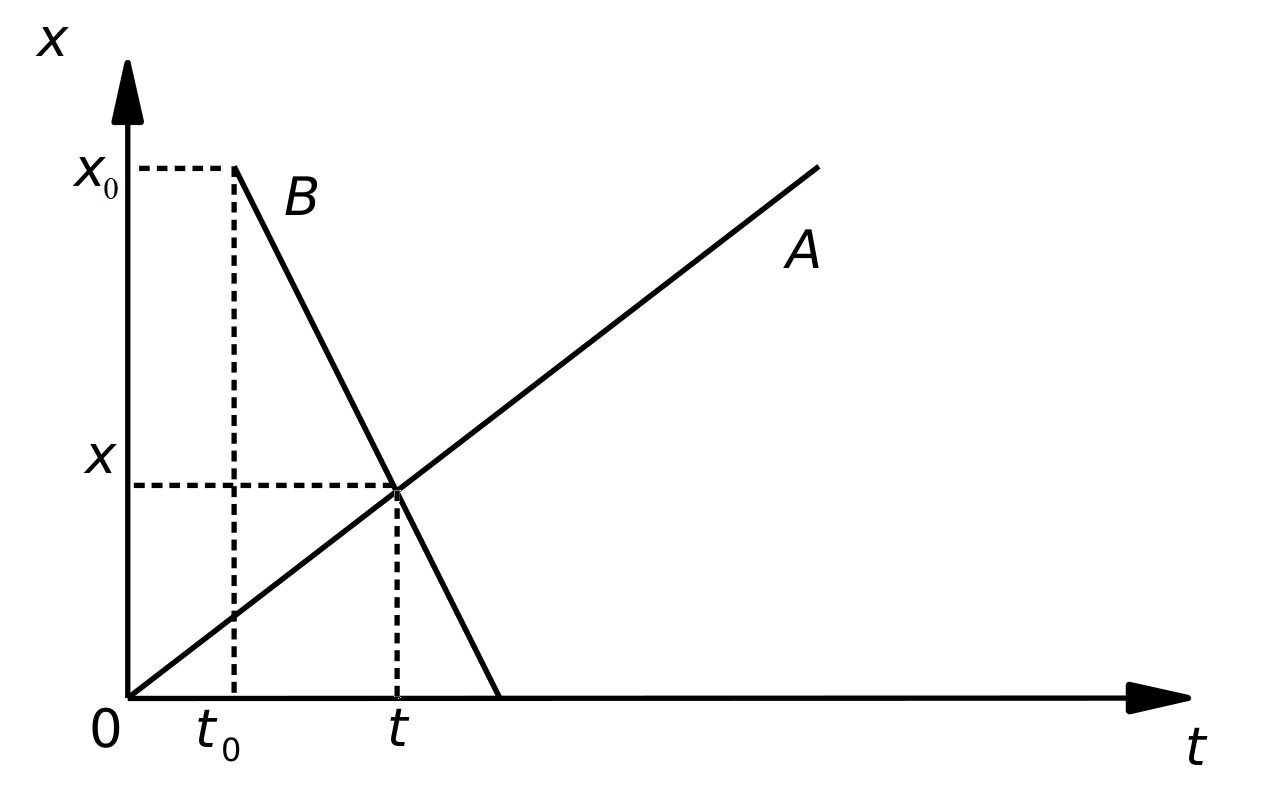
\includegraphics[width=0.6\textwidth]{38p40}
%\end{figure}
%\newline
%Als we voor $x$ de ontmoetingsplaats van $400\rm\,m$ nemen, hebben we twee vergelijkingen (\ref{verg A}), (\ref{verg B}) en twee onbekenden $t$, $v_a$. Dit kunnen we oplossen door een variabele te substitueren. We nemen de tijd, $(\ref{verg A})\Leftrightarrow t=\frac{x}{v_a}$ en substitueren deze in vergelijking (\ref{verg B}):
%\begin{eqnarray*}
%x&=&x_0-2v_a(t-t_0)\\
%&=&x_0-2v_a\left(\frac{x}{v_a}-t_0\right)\\
%&\Updownarrow&\\
%v_a&=&\frac{3x-x_0}{2t_0}=1,0\rm\,m/s
%\end{eqnarray*}
%En de snelheid van B:
%\begin{equation}
% v_b=-2v_a=\frac{x_0-3x}{t_0}=-2,0\rm\,m/s
%\end{equation} 
%\end{oplossing}


\end{exercise}

\begin{exercise} Een vliegtuig moet minstens een snelheid van $108\rm\,km/h$ hebben om te kunnen opstijgen. Indien de schroeven aan het toestel een versnelling van $1,50\rm\,m/s^2$ geven, hoe lang moet de startbaan dan minstens zijn? 
%\begin{oplossing}
%\footnote{$x=\frac{v^2}{2a}=300\rm\,m$}
%\end{oplossing}
\begin{oplossing}
\item[gegeven]$v=30,0\rm\,m/s$\newline$a=1,50\rm\,m/s^2$
\item[gevraagd]$x$
\item[oplossing]Doordat we de versnelling van het vliegtuig kennen en de snelheid die het moet bereiken, kunnen we de tijd die het vliegtuig hiervoor nodig heeft, gemakkelijke berekenen met de formule $v=v_0+at$ voor de snelheid van een EVRB:
\begin{eqnarray*}
t=\frac{v}{a}
\end{eqnarray*}
De afstand die in deze tijd wordt afgelegd, kunnen we berekenen doordat we de gemiddelde snelheid kennen\footnote{De benodigde afstand kunnen we evenzeer berekenen met de formule $x=x_0+v_0+\frac{1}{2}at^2$ door de tijd in te vullen.}:
\begin{eqnarray*}
x&=&\frac{v_0+v}{2}\cdot t\\
&=&\frac{v}{2}\cdot\frac{v}{a}\\
&=&\frac{v^2}{2a}
\end{eqnarray*}
De startbaan moet dus minstens $300\rm\,m$ lang zijn.
\end{oplossing}

\end{exercise}

\begin{exercise} Op een bevroren meer komt een glijdende hockeyschijf na $200\rm\,m$ tot stilstand. Als zijn initi\"ele snelheid $3,00\rm\,m/s$ was, bepaal dan
\begin{enumerate}
\item de versnelling in de veronderstelling dat deze constant is,
\item de tijd die de schijf nodig heeft om tot stilstand te komen.
\end{enumerate}
\begin{oplossing}
	$a=\frac{v_0^2}{2x}=0,0225\rm\,m/s^2$; $t=\frac{2x}{v_0}=133,33\rm\,s$
\end{oplossing}

\end{exercise}

\begin{exercise} Een bootje vaart met een snelheid van $36,0\rm\,km/h$ een eerste tijdopnemer voorbij en drijft daarna eenparig zijn snelheid op. Na $20,0\rm\,s$ komt het voorbij een tweede tijdopnemer met een snelheid van $90,0\rm\,km/h$. Bereken de versnelling van het bootje en de afstand tussen beide tijdopnemers.
\begin{oplossing}
\newline
$a=\frac{v-v_0}{t-t_0}=0,750\rm\,m/s^2$, $x-x_0=\left(\frac{v_0+v}{2}\right)(t-t_0)=350\rm\,m$
\end{oplossing}

\end{exercise}

\begin{exercise} Een auto begint te remmen als hij zich $35\rm\,m$ van een hindernis bevindt. Zijn snelheid op dat moment is $54\rm\,km/h$. Na $4,0\rm\,s$ botst hij tegen de hindernis. Bereken de snelheid waarmee hij de hindernis raakt en zijn constante versnelling gedurende de remweg.
\begin{oplossing}
$a=\frac{2(x-v_0t)}{t^2}=-3,125\rm\,m/s^2$, $v=\frac{2x}{t}-v_0=2,5\rm\,m/s$
\end{oplossing}
\begin{oplossing}
\item[gegeven]$x=35\rm\,m$\newline$v_0=15\rm\,m/s$\newline$t=4,0\rm\,s$
\item[gevraagd]$a, v$
\item[oplossing]Uit de plaatsfunctie kunnen we de versnelling halen:
\begin{eqnarray*}
x&=&v_0t+\frac{1}{2}at^2\\
&\Updownarrow&\\
a&=&\frac{2x-2v_0t}{t^2}
\end{eqnarray*}
Substitutie van de versnelling in de snelheidsfunctie levert:\footnote{Een andere (snellere) mogelijkheid is de snelheid uit $x=\frac{v_0+v}{2}t$ halen.}
\begin{eqnarray*}
v&=&v_0+at\\
&=&v_0+\left(\frac{2x-2v_0t}{t^2}\right)t\\
&=&\frac{2x}{t}-v_0\\
&=&2,5\rm\,m/s
\end{eqnarray*}
\end{oplossing}

\end{exercise}

\begin{exercise} Twee fietsers vertrekken gelijktijdig om
een afstand van $200\rm\,m$ af te leggen. De eerste rijdt met een
constante snelheid van $4,0\rm\,m/s$, terwijl de tweede vertrekt met
een snelheid van $1,00\rm\,m/s$ en de afstand van $200\rm\,m$ met
een EVRB met een versnelling van $0,20\rm\,m/s^2$ aflegt. Waar zal
de tweede fietser de eerste inhalen en wanneer?
\begin{oplossing}
\newline
$t=\frac{2(v_a-v_{b,0})}{a}=30\rm\,s$,
$x=v_at=\frac{2v_a(v_a-v_{b,0})}{a}=120\rm\,m$
\end{oplossing}

\end{exercise}

\begin{exercise} Laat zien dat voor een EVRB de volgende formules gelden:
\begin{eqnarray*}
x-x_0=\left(\frac{v+v_0}{2}\right)(t-t_0)\\
v^2=v_0^2+2a(x-x_0)\\
x-x_0=v(t-t_0)-\frac{1}{2}a(t-t_0)^2
\end{eqnarray*}

\end{exercise}

\begin{exercise} Een trein verlaat het station a en rijdt
naar het station b, op $15,0~\rm km$ van a gelegen. De eerste
$1000~\rm m$ worden afgelegd met een EVRB en de verkregen snelheid
is $72,0~\rm km/h$. Die snelheid blijft constant tot op $250~\rm m$
van b. Hier begint de trein te vertragen. Wanneer komt hij in
station b toe? Maak de $v(t)$-grafiek.










\end{exercise}

\begin{exercise} 
\begin{minipage}[t]{0.5\textwidth}
Een deeltje beschrijft een eendimensionale beweging op de $x$-as. De positie als functie van de tijd is hiernaast weergegeven in een $x(t)$-diagram. Duid de onderstaande grafiek aan die het best het verloop weergeeft van de snelheidscomponent $v$ van dat deeltje als functie van de tijd. 
\end{minipage}
\hspace{0.1\textwidth}
\begin{minipage}[t]{0.3\textwidth}
\raisebox{-5cm}{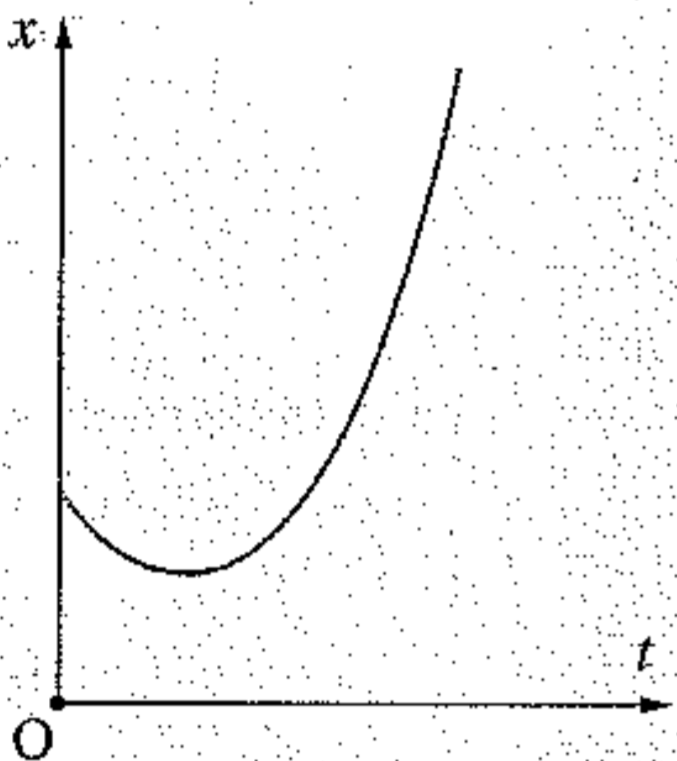
\includegraphics[width=\textwidth]{snelheidsverloop_o}}
\end{minipage}
\begin{figure}[h]
\begin{flushright}
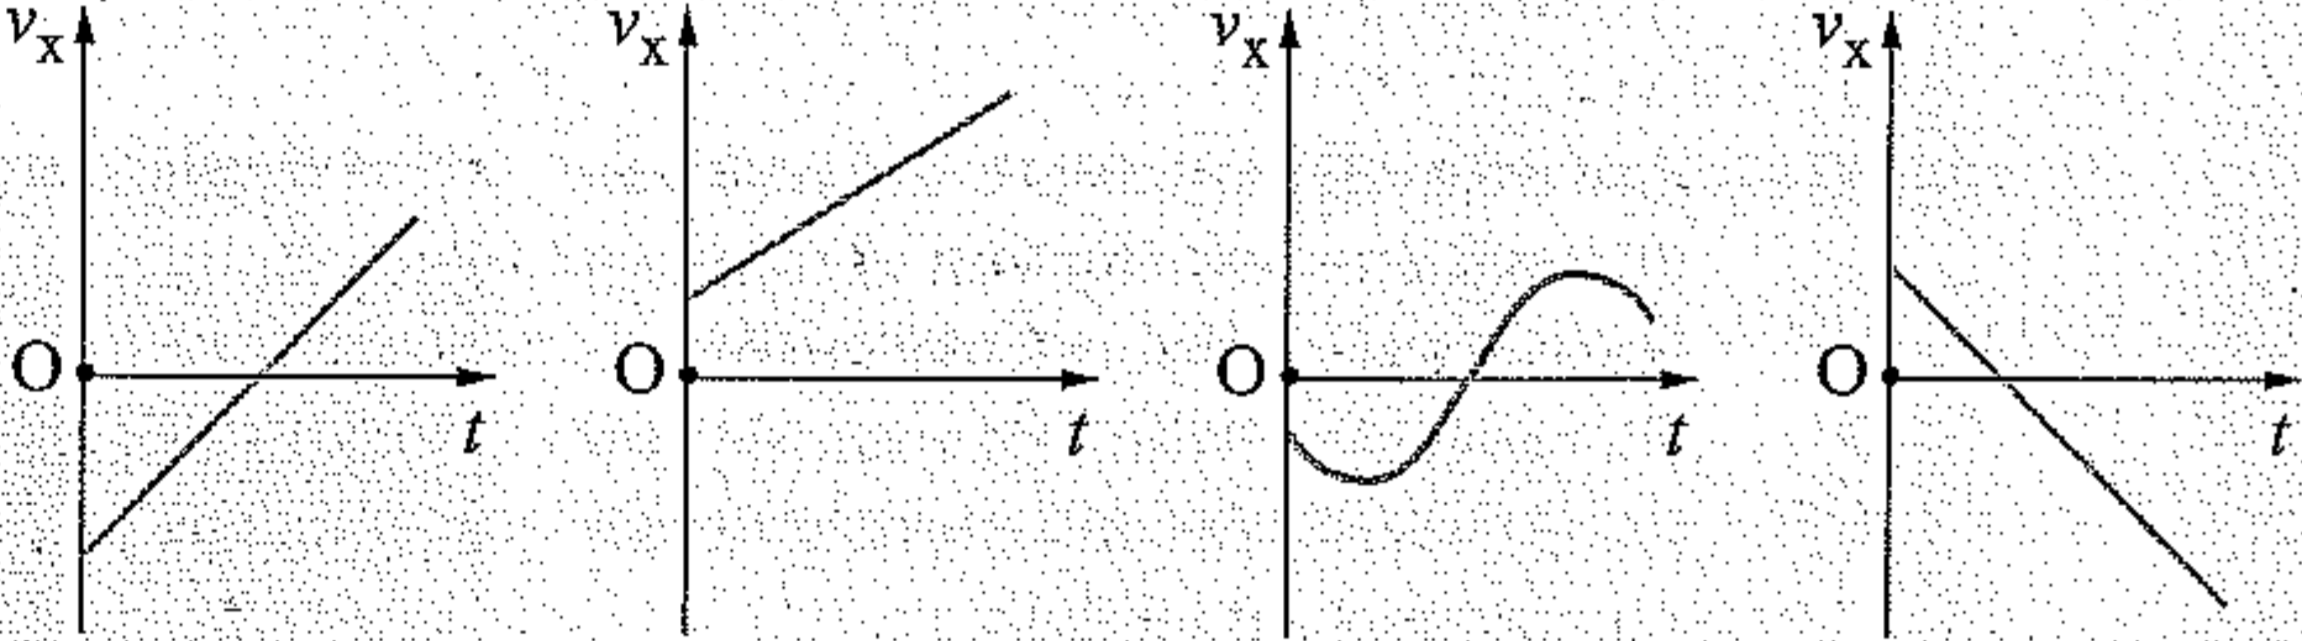
\includegraphics[width=0.93\textwidth]{snelheidsverloop}
\end{flushright}
\end{figure}

\end{exercise}

\begin{exercise} 
\begin{minipage}[t]{0.6\textwidth}
Een deeltje beweegt in de zin van de $x$-as. De nevenstaande grafiek geeft aan hoe de grootte van de snelheid verandert als functie van de tijd.
\begin{enumerate}
\item De afstand afgelegd na $15\rm\,s$ bedraagt:
\newline
\begin{tabularx}{\textwidth}{XXXX}
$30\rm\,m$&$120\rm\,m$&$150\rm\,m$&$240\rm\,m$
\end{tabularx}
\item Na $30\rm\,s$ heeft het deeltje een welbepaalde afstand afgelegd. Hoe groot zou de constante snelheid van het deeltje moeten zijn om in $30\rm\,s$ dezelfde afstand af te leggen?
\newline
\begin{tabularx}{\textwidth}{XXXX}
$0,0\rm\,m/s$&$§6,0\rm\,m/s$&$8,0\rm\,m/s$&$12\rm\,m/s$
\end{tabularx}
\end{enumerate}
\end{minipage}
\hspace{2mm}
\begin{minipage}[t]{0.3\textwidth}
\raisebox{-5cm}{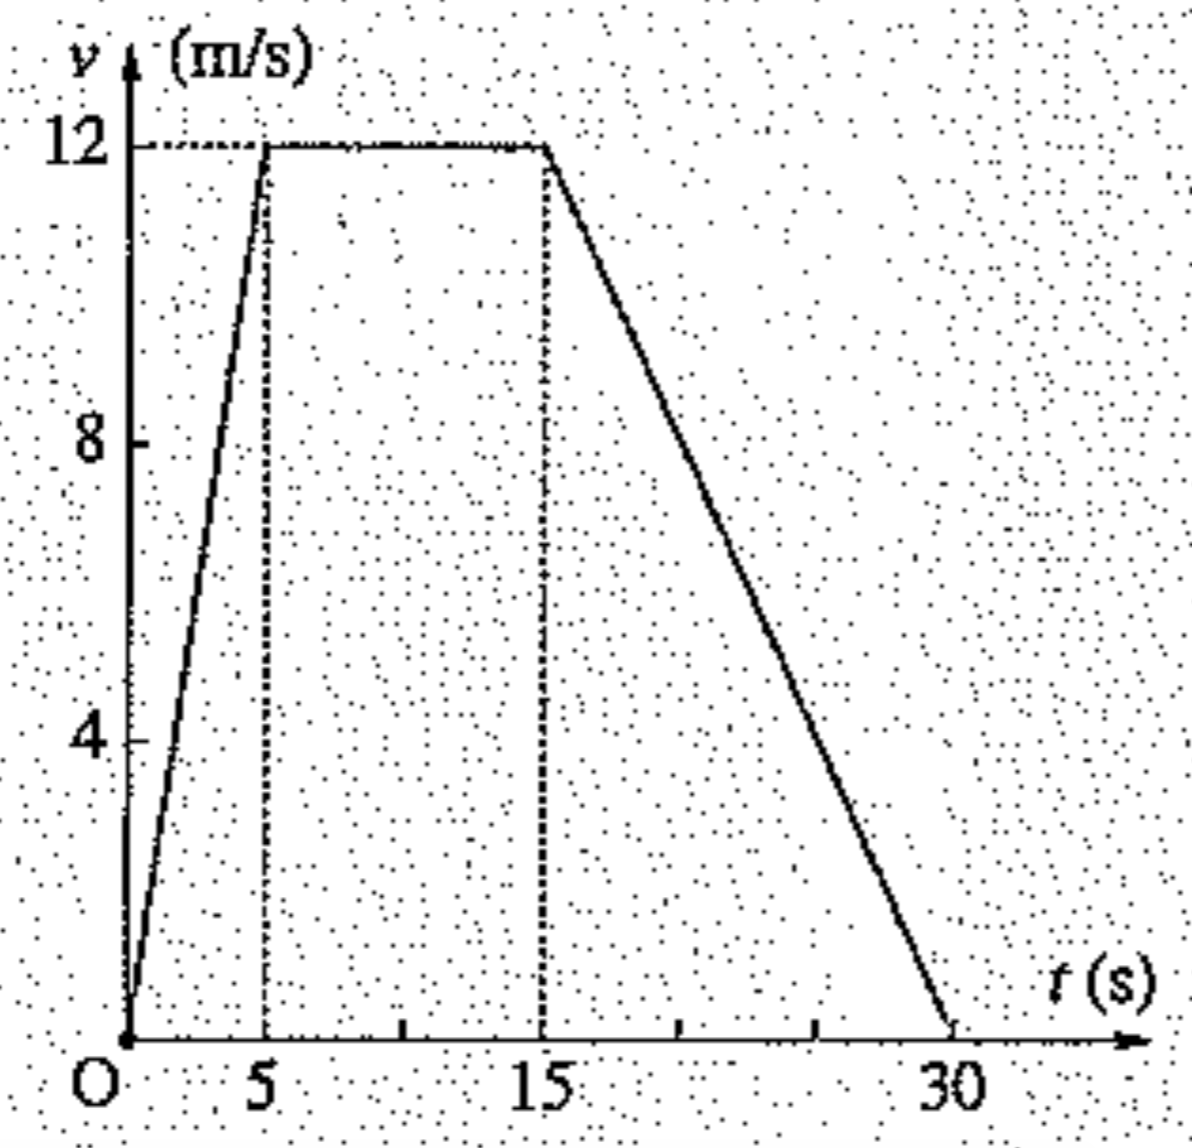
\includegraphics[width=\textwidth]{snelheidsverloop_2_o}}
\end{minipage}
\begin{enumerate}
\setcounter{enumii}{2}
\item Het verloop van de versnellingscomponent van het deeltje wordt kwalitatief voorgesteld op figuur:
\begin{figure}[h]
\begin{flushright}
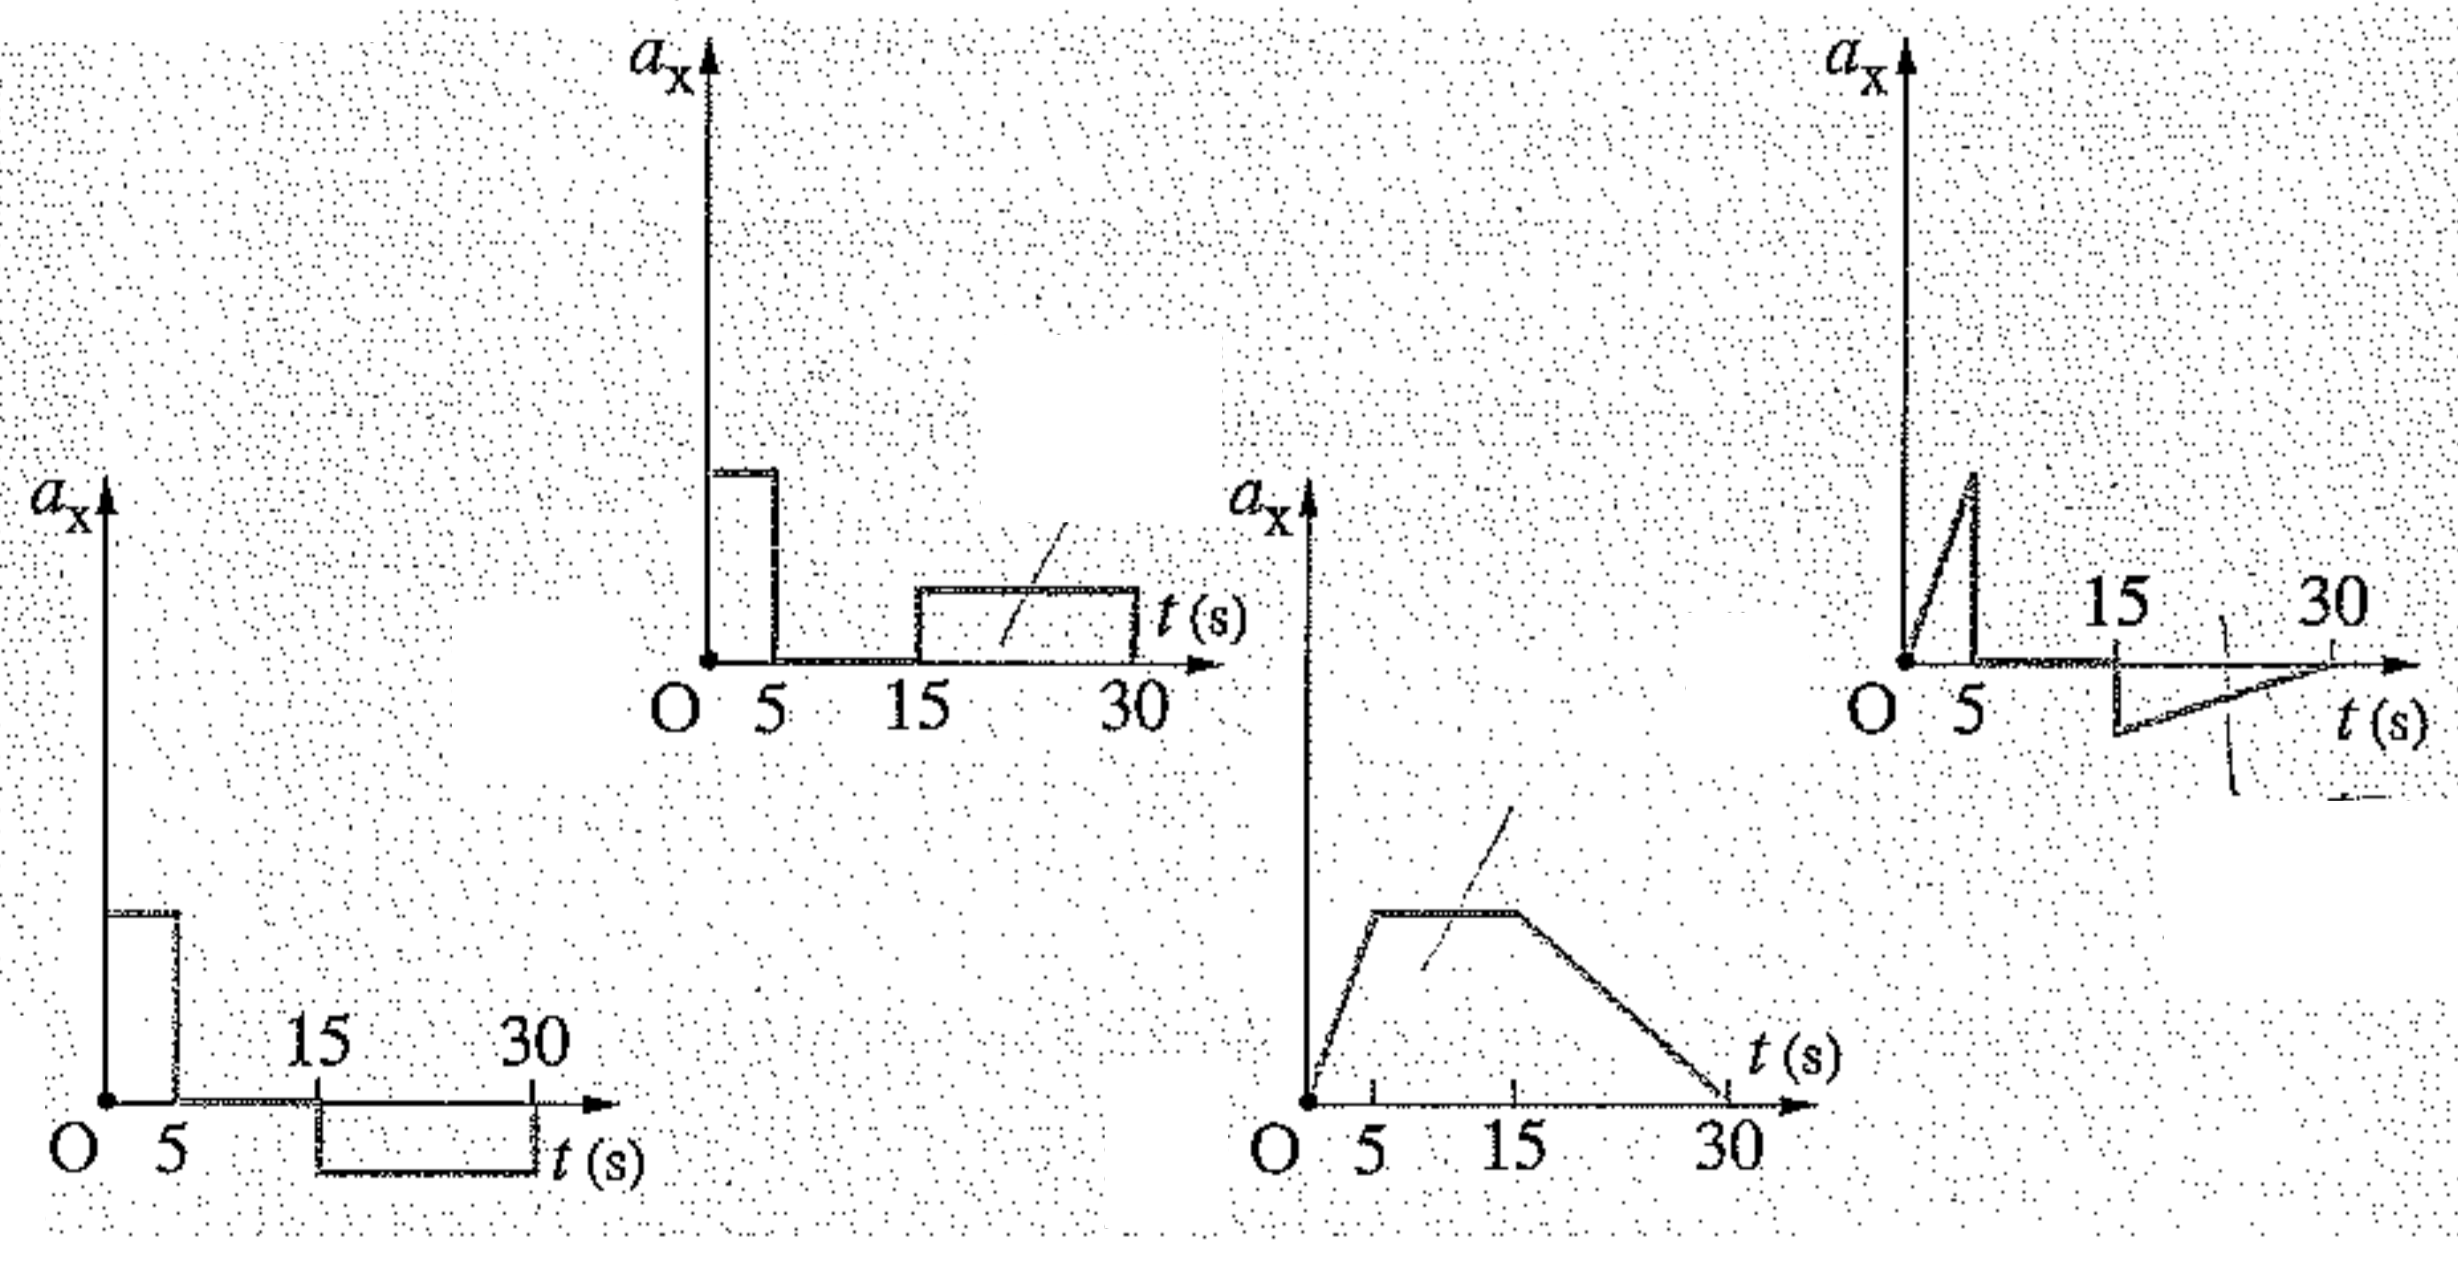
\includegraphics[width=0.93\textwidth]{snelheidsverloop_2}
\end{flushright}
\end{figure}
\end{enumerate}

\end{exercise}

\begin{exercise} Toon aan dat voor het stoptraject ($x_s$) van een auto de volgende vergelijking geldt:
\begin{eqnarray*}
x_s&=&v_0t_r-\frac{v_0^2}{2a}
\end{eqnarray*}
waarin $v_0$ de beginsnelheid van de auto is, $t_r$ de reactietijd van de bestuurder, en $a$ de vertraging (negatief).
\newline
\newline
Maak een $x(t)-,\,v(t)-$ en een $a(t)-$grafiek van de beweging.
\begin{oplossing}
\newline
\newline
Het stoptraject bestaat uit twee delen: gedurende de reactietijd blijft de bestuurder met de gegeven snelheid verder rijden om vervolgens, van zodra hij de rem indrukt, effectief te beginnen remmen. Het stoptraject bestaat uit de som van de afstanden afgelegd gedurende die twee delen:
\begin{eqnarray*}
x_s=\Delta x_{\mathrm{reactie}}+\Delta x_{\mathrm{rem}}
\end{eqnarray*}
Omdat de snelheid gedurende de reactietijd constant is, wordt de afstand die hier wordt afgelegd gegeven door $\Delta x_{\mathrm{reactie}}=v_0t_r$. In het tweede deel bestaat de beweging uit een rechtlijnige beweging met een constante versnelling. Omdat de tijd om van een gegeven snelheid tot stilstand te komen, wordt gegeven door $\Delta t=-\frac{v_0}{a}$ en de gemiddelde snelheid door $\frac{v_0}{2}$, wordt de afstand gegeven door $\Delta x_{\mathrm{rem}}=\bar{v}\Delta t=-\frac{v_0}{a}\frac{v_0}{2}=-\frac{v_0^2}{2a}$. We vinden het stoptraject als de som van de twee afstanden.
%$\Delta x_{rem}=v_0\Delta t+\frac{1}{2}a\Delta t^2$.
\end{oplossing}



\end{exercise}

\begin{exercise} (III) Maggie en Jennifer lopen de \SI{100}{m}. Beiden doen ze er exact 10,2 se\-conden over. Met een eenparige versnelling bereikt Maggie na \SI{2}{s} haar maximale snelheid, Jennifer doet dat na \SI{3}{s}. Hun maximale snelheden houden ze aan voor de rest van de wedstrijd.
\begin{enumerate}
\item Wat zijn hun maximale snelheden?
\item Wat is de versnelling van iedere sprinter?
\item Wie heeft er voorsprong na \SI{6}{s}, en hoeveel?
\end{enumerate}
\begin{oplossing}
\footnote{antw. $v_1=\frac{2x_2}{2t_2-t_1}$;
$a=\frac{2x_2}{(2t_2-t_1)t_1}$;
$x_M-x_J=\frac{2x_2}{2t_2-t_{1,M}}(t-\frac{t_{1,M}}{2})-\frac{2x_2}{2t_2-t_{1,J}}(t-\frac{t_{1,J}}{2})$}
\end{oplossing}

\end{exercise}

\begin{exercise} Welke afstand wordt er door een bungeespringer na een vrije val van $2,5\rm\,s$ afgelegd?
\begin{oplossing}
\footnote{$x=\frac{1}{2}gt^2=31\rm\,m$}
\end{oplossing}







\end{exercise}

\begin{exercise} Men laat een steen vallen van een $44,1\rm\,m$ hoge brug. $1\rm\,s$ later werpt men een tweede steen verticaal naar beneden. Beide raken gelijk het wateroppervlak. Zoek de beginsnelheid van de tweede steen.
\begin{oplossing}
\footnote{antw. $12,26\rm\,m/s$}
\end{oplossing}












\end{exercise}

\begin{exercise} (III) Germien laat een steen in een diepe put vallen. Na 2,6 seconden hoort ze dat de steen de bodem heeft geraakt. Hoe diep is de put? Neem voor de snelheid van het geluid $343\rm\,m/s$.




\begin{oplossing}
\begin{enumerate}
\item[\textit{gegeven}]$v_0=50\rm\,m/s$\newline$a=-30\rm\,m/s^2$\newline$v=5,0\rm\,m/s$
\item[\textit{gevraagd}]$x$
\item[\textit{oplossing}]Aangezien we de versnelling en begin- en eindsnelheid kennen, kunnen we de tijd die nodig is om de eindsnelheid te bereiken, berekenen:
\begin{eqnarray*}
v=v_0+at&\Leftrightarrow&t=\frac{v-v_0}{a}
\end{eqnarray*}
De afgelegde afstand is dan met gemiddelde snelheid te bepalen:
\begin{eqnarray*}
x&=&\overline{v}t\\
&=&\frac{v_0+v}{2}\cdot\frac{v-v_0}{a}\\
&=&\frac{v^2-v_0^2}{2a}\\
&=&41,25\rm\,m
\end{eqnarray*}
\end{enumerate}
\end{oplossing}
	



\end{exercise}

\begin{exercise} Een auto die $90\rm\,km/h$ rijdt, ligt $100\rm\,m$ achter op een vrachtwagen die $75\rm\,km/h$ rijdt. Hoeveel tijd kost het de auto om de vrachtwagen in te halen? 
\begin{oplossing}
\footnote{$t=\frac{x_0}{v_a-v_v}=24\rm\,s$}
\end{oplossing}

\end{exercise}

\begin{exercise} De snelheid van een trein verandert eenparig in 2 minuten van $20\rm\,km/h$ tot $30\rm\,km/h$. De trein rijdt gedurende die tijd over een rechte spoorlijn.
\begin{enumerate}
    \item Bepaal de versnelling.
    \item Bepaal de afstand die de trein heeft afgelegd gedurende deze 2 minuten.
\end{enumerate}

\end{exercise}

\begin{exercise} Een auto trekt in $5,0\rm\,s$ op van $10\rm\,m/s$ naar $25\rm\,m/s$. Wat was de versnelling in de veronderstelling dat de auto een EVRB ondergaat? Welke afstand legde de auto in deze periode af?
\begin{oplossing}
\newline
$a=\frac{v-v_0}{t-t_0}=3\rm\,m/s$,
$x-x_0=\left(\frac{v_0+v}{2}\right)(t-t_0)=87,5\rm\,m$
\end{oplossing}

\end{exercise}

\begin{exercise} Bij het katapulteren van vliegtuigen wordt een startbaan van
$25,0\rm\,m$ gebruikt, die door het vliegtuig eenparig versneld in
$1,00\rm\,s$ wordt doorlopen. Zoek zijn versnelling en de snelheid
waarmee het de baan verlaat.

\end{exercise}

\begin{exercise} Een auto trekt op tot $100\rm\,km/h$ in $6,0\rm\,s$. Als hij
dat doet op een rechte baan met constante versnelling, welke afstand
is er dan hiervoor nodig?~\footnote{antw.
$a=\frac{v}{t}=4,63\rm\,m/s^2$, $x=\frac{vt}{2}=83,3\rm\,m$}

\end{exercise}

\begin{exercise} Een auto vertrekt vanuit rust en bereikt na $3,0\rm\,km$ een snelheid van $450\rm\,km/h$ We onderstellen de versnelling constant en de baan recht. Bereken de versnelling en de tijd, nodig om die $3,0\rm\,km$ af te leggen.
\begin{oplossing}
\footnote{$t=\frac{2x}{v}=48\rm\,s$, $a=\frac{v^2}{2x}=2,6\rm\,m/s^2$}
\item[gegeven]$x=3000\rm\,m$\newline $v=125\rm\,m/s$
\item[gevraagd]$a$, $t$
\item[oplossing]Omdat voor een EVRB de gemiddelde snelheid gegeven wordt door $\overline{v}=\frac{v_0+v}{2}$ en we de afgelegde afstand kennen, kunnen we de benodigde tijd gemakkelijk vinden. We kiezen $t_0=0$, $x_0=0$. De beginsnelheid is nul zodat:
\begin{eqnarray*}
\Delta x &=& \overline{v}\Delta t \\
&\Downarrow & \\
t &=& \frac{x}{\left(\frac{v}{2}\right)} = \frac{2x}{v}
\end{eqnarray*}
Invullen van de gegevens levert een tijd van $48\rm\,s$. Met het formuletje voor de snelheid vinden we de versnelling door de tijd te substitueren:
\begin{eqnarray*}
v &=& at \\
&\Updownarrow&\\
a &=& \frac{v}{t}=\frac{v}{\left(\frac{2x}{v}\right)}\\
&=& \frac{v^2}{2x}
\end{eqnarray*}
Invullen van de gegeven grootheden levert een versnelling van $2,6\rm\,m/s^2$.
\end{oplossing}

\end{exercise}

\begin{exercise} Een vliegtuig landt met een snelheid van $100\rm\,m/s$. Op de ladingsbaan heeft het een vertraging van $5,0\rm\,m/s^2$. Welke afstand heeft het vliegtuig nodig om tot stilstand te komen?

\end{exercise}

\begin{exercise} Een trein vertrekt uit een station en rijdt met een eenparig
versnelde beweging waarvan de versnelling $0,50\rm\,m/s^2$ bedraagt.
Hoe groot is de afstand die de trein heeft afgelegd als zijn
snelheid $72,0\rm\,km/h$ bedraagt?



\end{exercise}

\begin{exercise} Een puntmassa voert een eenparig veranderlijke rechtlijnige
beweging uit over het tijdsinterval [$0\rm\,s$,$2\rm\,s$] met
beginsnelheid en beginpositie van respectievelijk $0\rm\,m/s$ en
$0\rm\,m$. De versnelling is $3\rm\,m/s^2$. Waarom kan je
onmiddellijk stellen dat als in het tijdsinterval de tijd half om
is, de puntmassa nog niet halfweg is?
\begin{enumerate}
    \item Breng, zoals de opgelegde werkwijze bij het oplossen van
    vraag\-stuk\-ken vereist, zowel het gegeven als het gevraagde (hier
    het te bewijzen) in symbolen.
    \item Leg in woorden uit op welke manier je onmiddellijk kan
    inzien dat het te bewijzen juist is.
    \item Controleer het te bewijzen via de numerieke waarden van
    dit vraagstuk.
    \item Geef nu het bewijs.
\end{enumerate}

\end{exercise}

\begin{exercise} Een puntmassa beweegt volgens een eenparig veranderlijke
rechtlijnige beweging. De puntmassa heeft een beginsnelheid $v_0$ en
een snelheid $v$ op het tijdstip $t$. Wat is zijn gemiddelde
snelheid over het interval [0,$t$]?

\end{exercise}

\begin{exercise} Een sprinter legt de 100 meter af in
$12,0~\rm s$. Het snelheidsverloop van de sprinter is in
onderstaande figuur grafisch voorgesteld.
\begin{figure}[h]
\begin{center}
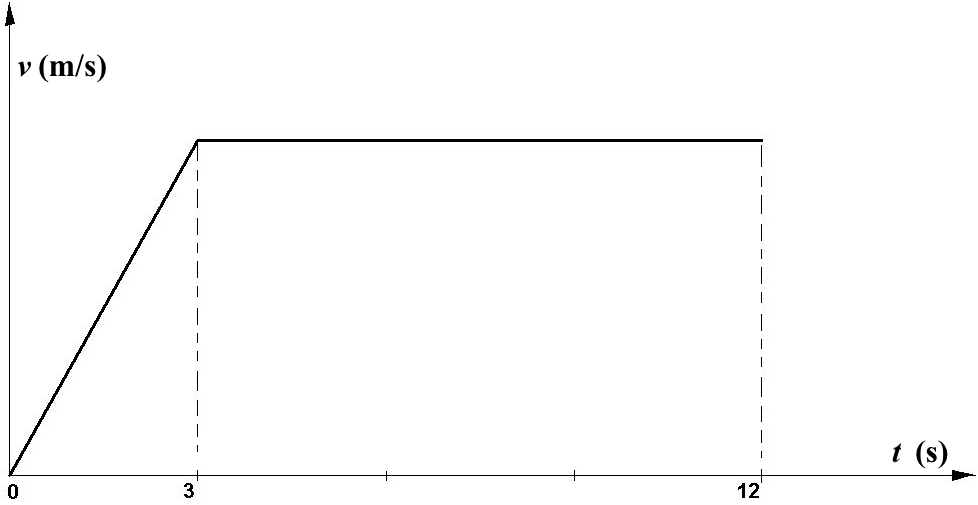
\includegraphics[width=0.5\textwidth, angle=0]{sprinter}
\end{center}
\end{figure}
\newline
Bereken
\begin{enumerate}
\item de constante snelheid die de sprinter gedurende de laatste 9
seconden aanhoudt,
\item de afstand die de sprinter gedurende de eerste 3 seconden
aflegt,
\item de versnelling die de sprinter heeft gedurende de eerste 3 seconden.
\end{enumerate}

\end{exercise}

\begin{exercise} Een ruimtevoertuig met een constante versnelling verhoogt
zijn snelheid van $65\rm\,m/s$ op $t=0\rm\,s$, tot $162\rm\,m/s$ op
$t=10,0\rm\,s$. Welke afstand legde dit voertuig af tussen
$t=2,0\rm\,s$ en $t=6,0\rm\,s$?~\footnote{antw.
$x_2-x_1=v_0(t_2-t_1)+\frac{1}{2}\left(\frac{v-v_0}{t}\right)(t_2^2-t_1^2)=415\rm\,m$}



\end{exercise}

\begin{exercise} Toon aan dat voor het stoptraject ($x_s$) van een auto de volgende vergelijking geldt:
%\begin{eqnarray*}
%x_s&=&v_0t_r-\frac{v_0^2}{2a}
%\end{eqnarray*}
%waarin $v_0$ de beginsnelheid van de auto is, $t_r$ de reactietijd van de bestuurder, en $a$ de vertraging (negatief).
%\newline
%\newline
%Maak een $x(t)-,\,v(t)-$ en een $a(t)-$grafiek van de beweging.

\end{exercise}

\begin{exercise} Een onopgemerkte politieauto met
een constante snelheid van 90 km/h wordt ingehaald door een
snelheidsovertreder die 144 km/h rijdt. Precies 1,00 s nadat de
snelheidsovertreder passeert, geeft de politieagent plankgas; stel
dat de politieauto een versnelling heeft van $2,00\rm\,m/s^2$.
\begin{enumerate}
\item Hoe lang duurt het voordat de agent de snelheidsovertreder
(die met een constante snelheid blijft rijden) heeft ingehaald?
\item Wat is zijn snelheid op dat moment?
\item Schets nauwkeurig en net de $x(t)-,v(t)-$ en $a(t)-$grafieken.
Behandel de politieauto en de overtreder steeds in dezelfde grafiek.
\item Vind een (algebra\"ische) formule voor de gemiddelde snelheid $\overline{v}_{12}$ in
functie van de gegeven grootheden, tussen het tijdstip waarop de
agent begint te versnellen en het tijdstip waarop hij de overtreder
inhaalt.
\end{enumerate}

\end{exercise}

\begin{exercise} Een onopgemerkte politieauto met een constante snelheid van $95\rm\,km/h$ wordt ingehaald door een snelheidsovertreder die $140\rm\,km/h$ rijdt. Precies $1,00\rm\,s$ nadat de snelheidsovertreder passeert, geeft de politieagent plankgas; stel dat de politieauto een versnelling heeft van $2,00\rm\,m/s^2$, hoe lang duurt het dan voordat de agent de snelheidsovertreder (die met een constante snelheid blijft rijden) heeft ingehaald? 


\end{exercise}

\begin{exercise} Twee fietsers vertrekken gelijktijdig om een afstand van $500\rm\,m$ af te leggen. De eerste rijdt met een constante snelheid van $5,0\rm\,m/s$, terwijl de tweede het traject aflegt met een EVRB waarvan de beginsnelheid $1,0\rm\,m/s$ is en de versnelling $0,2\rm\,m/s^2$. Beantwoord de volgende vragen:
\begin{enumerate}
\item Waar zal de tweede fietser de eerste inhalen? 
\item Hoeveel tijd is er dan verstreken? 
\item Hoelang doet de `winnaar' over het traject en wat is zijn snelheid op het moment van aankomst?
\item Teken een grafiek met beide plaatsfuncties en daaronder een grafiek met beide snelheidsfuncties. 
\item Wat kan je zeggen over de gemiddelde snelheden gedurende het tijdsverloop dat de tweede nodig heeft om de eerste in te halen? Leg uit.
\item Is er gedurende dit tijdsverloop een tijdstip waarop de tweede een snelheid heeft die gelijk is aan de
gemiddelde snelheid van de eerste? Leg uit.
\end{enumerate}

\end{exercise}

\begin{exercise} Een auto trekt in $5,0\rm\,s$ op van $10\rm\,m/s$ naar $25\rm\,m/s$. Wat is de versnelling van de auto in de veronderstelling dat hij een EVRB ondergaat? Welke afstand legt de auto in deze periode af?

\end{exercise}

\begin{exercise} Een vliegtuig landt met een snelheid van $100\rm\,m/s$. Op de landingsbaan heeft het een vertraging van $5,0\rm\,m/s^2$. Welke afstand heeft het vliegtuig nodig om tot stilstand te komen? % gegevens nagaan?...

\end{exercise}

\begin{exercise} Een trein vertrekt uit een station en rijdt met een eenparig versnelde beweging waarvan de versnelling $0,50\rm\,m/s^2$ bedraagt. Hoe groot is de afstand die de trein heeft afgelegd als zijn snelheid $72,0\rm\,km/h$ bedraagt?

\end{exercise}

\begin{exercise} Kathy Koel en Stan Spidi fietsen over een afstand van $150\rm\,m$. Kathy houdt een constante snelheid van $5,00\rm\,m/s$ aan. Stan vertrekt met $2,00\rm\,m/s$, maar rijdt eenparig versneld.
\begin{enumerate}
\item Hoe groot moet de versnelling van Stan zijn opdat hij gelijktijdig met Kathy de eindmeet zou bereiken?
\item Hoe groot is de gemiddelde snelheid van Stan?
\end{enumerate}
\begin{oplossing}
\item[\textit{gegeven:}]$V_0=2,00\rm\,m/s$\newline$v_k=5,00\rm\,m/s$\newline$x=150\rm\,m$
\item [\textit{gevraagd:}]$a$, $\overline{v}$
\item [\textit{oplossing:}]
\begin{enumerate}
\item De tijd die Kathy nodig heeft om de
$150\rm\,m$ af te leggen is:
\begin{eqnarray*}
t=\frac{x}{v_k}
\end{eqnarray*}
Op dit tijdstip hebben beide $150\rm\,m$ afgelegd zodat:
\begin{eqnarray*}
x_k&=&x_s\\
&\Updownarrow&\\
v_kt&=&v_0t+\frac{1}{2}at^2\\
&\Updownarrow&\\
a&=&\frac{2(v_k-v_0)}{t}\\
&=&\frac{2v_k(v_k-v_0)}{x}\\
&=&0,200\rm\,m/s^2
\end{eqnarray*}
\item Aangezien Stan dezelfde afstand aflgegt als Kathy in dezelfde tijd, is
zijn gemiddelde snelheid gelijk aan de snelheid van Kathy:
\begin{eqnarray*}
\overline{v}=\frac{\Delta x}{\Delta t}=\frac{x}{t}=v_k
\end{eqnarray*}
\end{enumerate}
\end{oplossing}



\end{exercise}

\begin{exercise} Quick en Flupke bewegen volgens de volgende plaatsfuncties:
\begin{eqnarray*}
\mathrm{Quick:}&&x=x_0+v_qt+\frac{1}{2}at^2\\
\mathrm{Flupke:}&&x=x_0+v_ft
\end{eqnarray*}
waarbij $v_{q}$ en $v_{f}$ constante snelheden zijn en $x_0$ de gemeenschappelijke beginpositie op tijdstip $t_0=0$. Als je weet dat er een tijdstip t $(t>0)$ bestaat waarop beiden elkaar terug ontmoeten, beantwoord dan de volgende vragen:
\begin{enumerate}
\item Wat is de gemiddelde snelheid van Flupke gedurende het tijdsverloop $\Delta t=t-0=t$? 
\item Wat weet je over de gemiddelde snelheid van Quick gedurende hetzelfde tijdsverloop?
\item Vind een uitdrukking zonder plaatsaanduiding voor de versnelling van Quick. 
\item Indien de beginsnelheid van Quick groter is dan die van Flupke, wat kan je
dan zeggen over het teken van zijn versnelling? Leg uit. 
%\item Is er een moment waarop de snelheid van Quick negatief is?
%\item Vind een uitdrukking voor de tijd waarop de snelheid van Quick nul is in functie van zijn versnelling $a$. Zorg dat $a$ de enige afhankelijke variabele is in de uitdrukking. Haal hieruit het maximale tijdstip waarop zijn snelheid nul kan worden indien $a$ positief is.
\end{enumerate}

\end{exercise}

\begin{exercise} De snelheid van een deeltje voldoet aan $v=at$ waarin $a$ constant en negatief is. De plaats van het deeltje wordt voorgesteld door $x$. Aangenomen wordt dat $x=0\rm\,m$ op het ogenblik $t=0\rm\,s$. Welke grafiek geeft het juiste verloop van $x(t)$?
%\begin{figure}[h]
%\begin{flushright}
%\subimport{./Figuren/}{30p38_a.tex}\subimport{./Figuren/}{30p38_b.tex}\subimport{./Figuren/}{30p38_c.tex}\subimport{./Figuren/}{30p38_d.tex}
%%\caption{Caption}
%%\label{fig:my_label}
%\end{flushright}
%\end{figure}

\end{exercise}

\begin{exercise} 
%\begin{minipage}[t]{0.5\textwidth}
%Een deeltje beschrijft een eendimensionale beweging op de $x$-as. De positie als functie van de tijd is hiernaast weergegeven in een $x(t)$-diagram. Duid de onderstaande grafiek aan die het best het verloop weergeeft van de snelheidscomponent $v$ van dat deeltje als functie van de tijd. 
%\end{minipage}
%\hspace{0.1\textwidth}
%\begin{minipage}[t]{0.3\textwidth}
%\raisebox{-5cm}{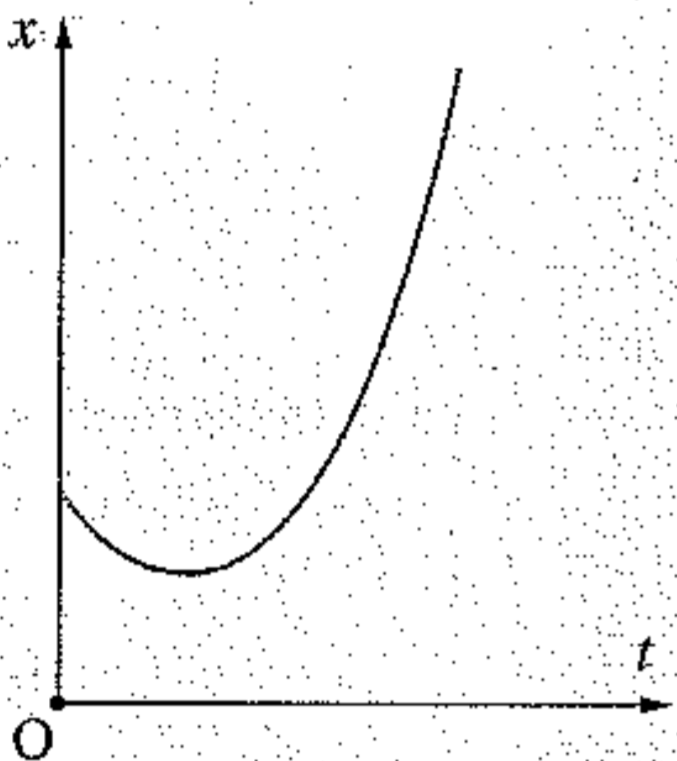
\includegraphics[width=\textwidth]{snelheidsverloop_o}}
%\end{minipage}
%\begin{figure}[H]
%\begin{flushright}
%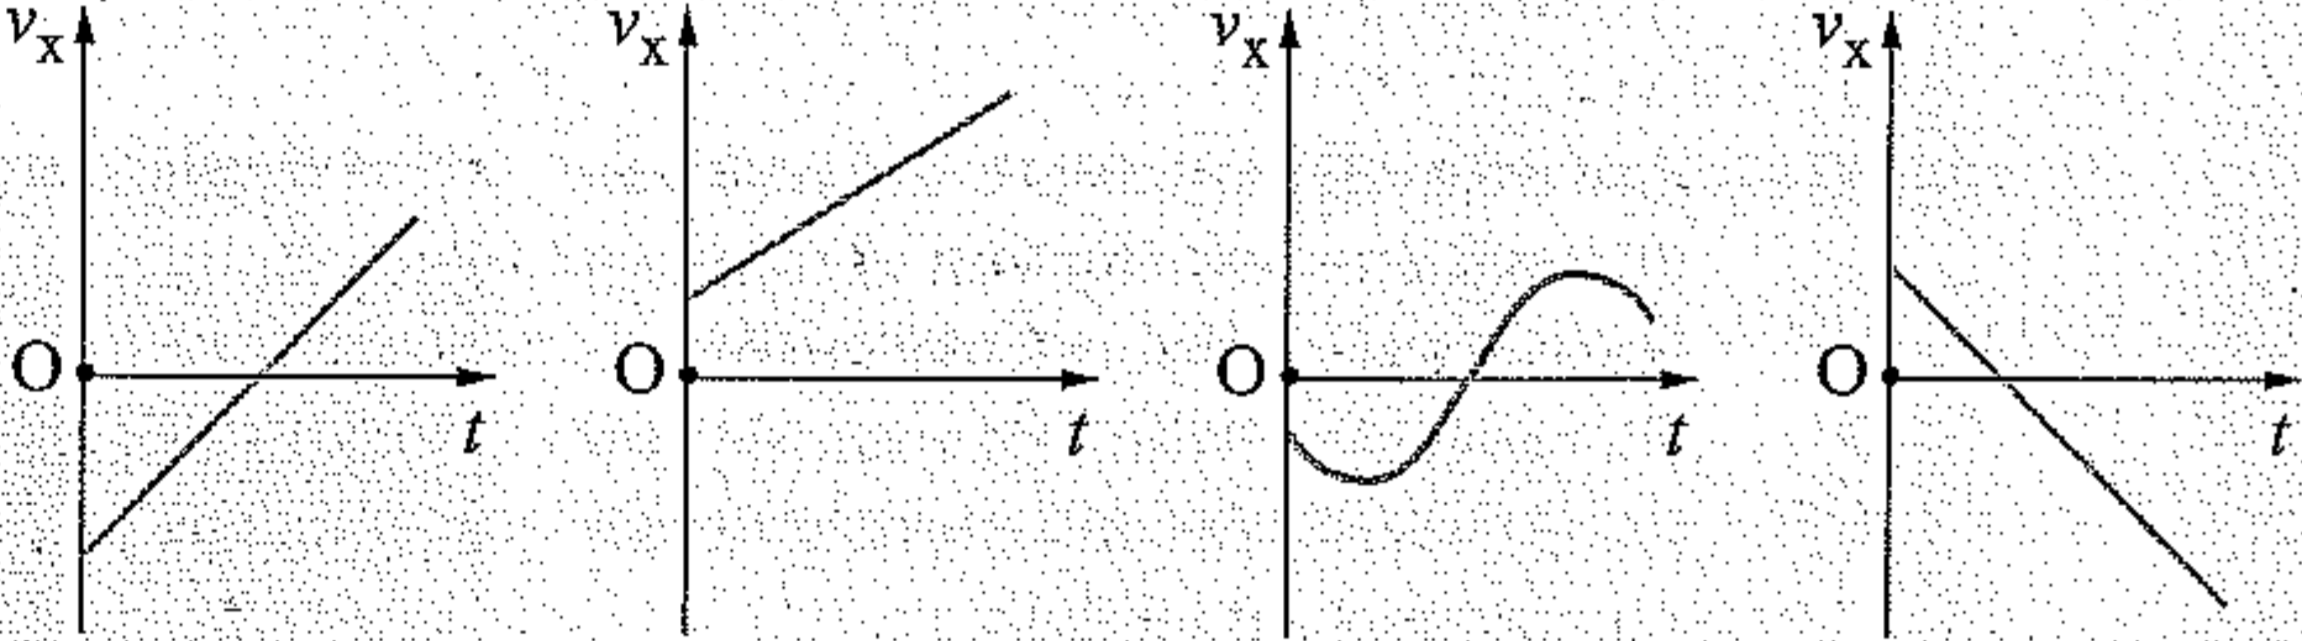
\includegraphics[width=0.93\textwidth]{snelheidsverloop}
%\end{flushright}
%\end{figure}

%\newpage

\end{exercise}

\begin{exercise} 
%\begin{minipage}[t]{0.6\textwidth}
%Een deeltje beweegt in de zin van de $x$-as. De nevenstaande grafiek geeft aan hoe de grootte van de snelheid verandert als functie van de tijd.
%\begin{enumerate}
\end{exercise}

\begin{exercise} De afstand afgelegd na $15\rm\,s$ bedraagt:
%\newline
%\begin{tabularx}{\textwidth}{XXXX}
%$30\rm\,m$&$120\rm\,m$&$150\rm\,m$&$240\rm\,m$
%\end{tabularx}
\end{exercise}

\begin{exercise} Na $30\rm\,s$ heeft het deeltje een welbepaalde afstand afgelegd. Hoe groot zou de constante snelheid van het deeltje moeten zijn om in $30\rm\,s$ dezelfde afstand af te leggen?
%\newline
%\begin{tabularx}{\textwidth}{XXXX}
%$0,0\rm\,m/s$&$§6,0\rm\,m/s$&$8,0\rm\,m/s$&$12\rm\,m/s$
%\end{tabularx}
%\end{enumerate}
%\end{minipage}
%\hspace{2mm}
%\begin{minipage}[t]{0.3\textwidth}
%\raisebox{-5cm}{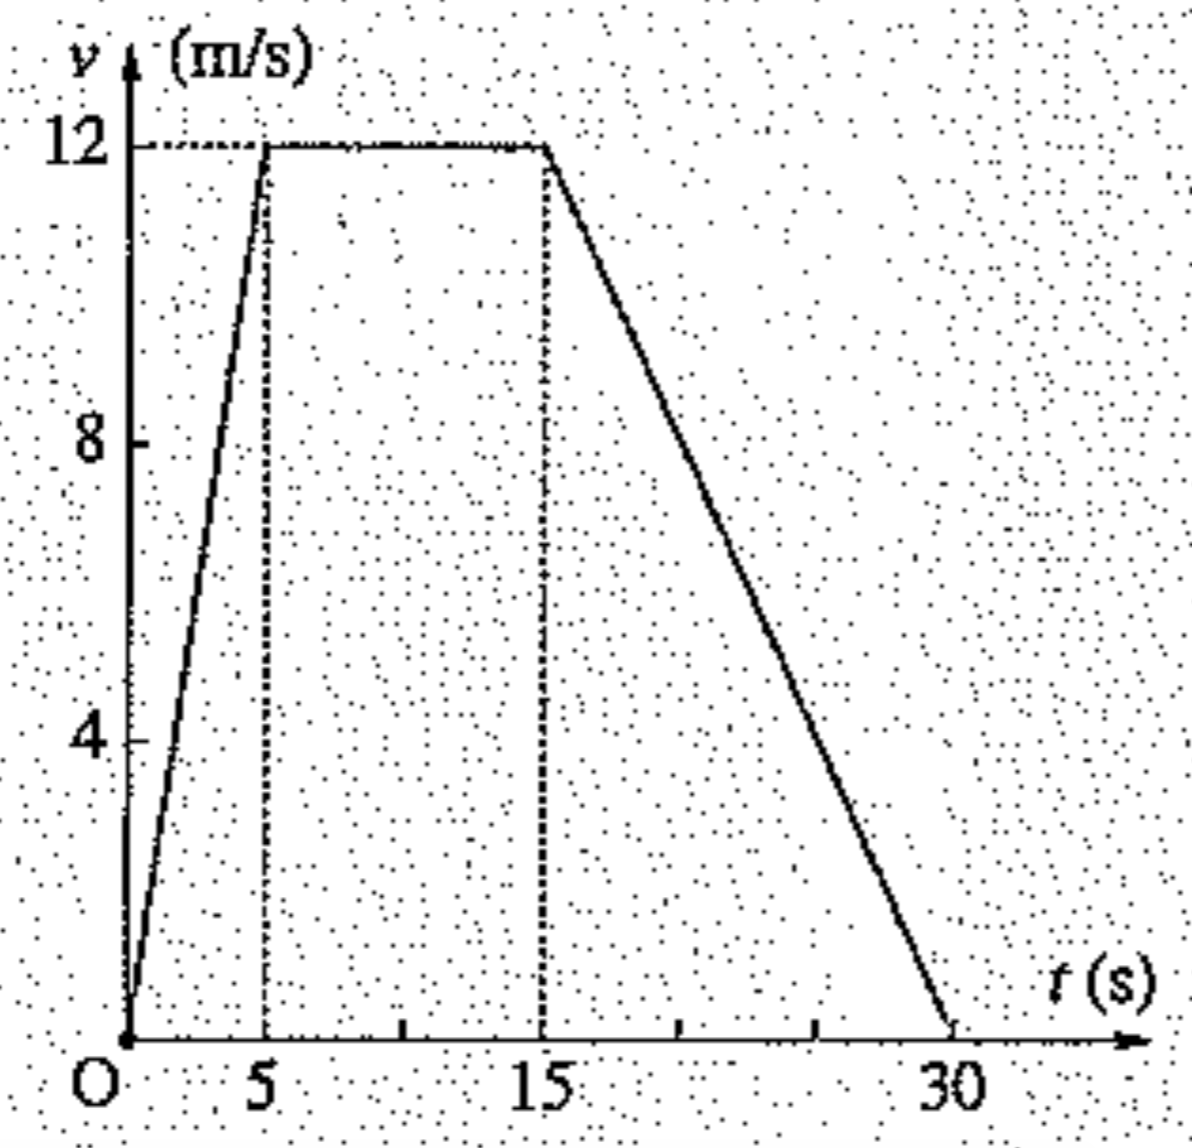
\includegraphics[width=\textwidth]{snelheidsverloop_2_o}}
%\end{minipage}
%\begin{enumerate}
%\setcounter{enumii}{2}
\end{exercise}

\begin{exercise} Het verloop van de versnellingscomponent van het deeltje wordt kwalitatief voorgesteld op figuur:
%\begin{figure}[H]
%\begin{flushright}
%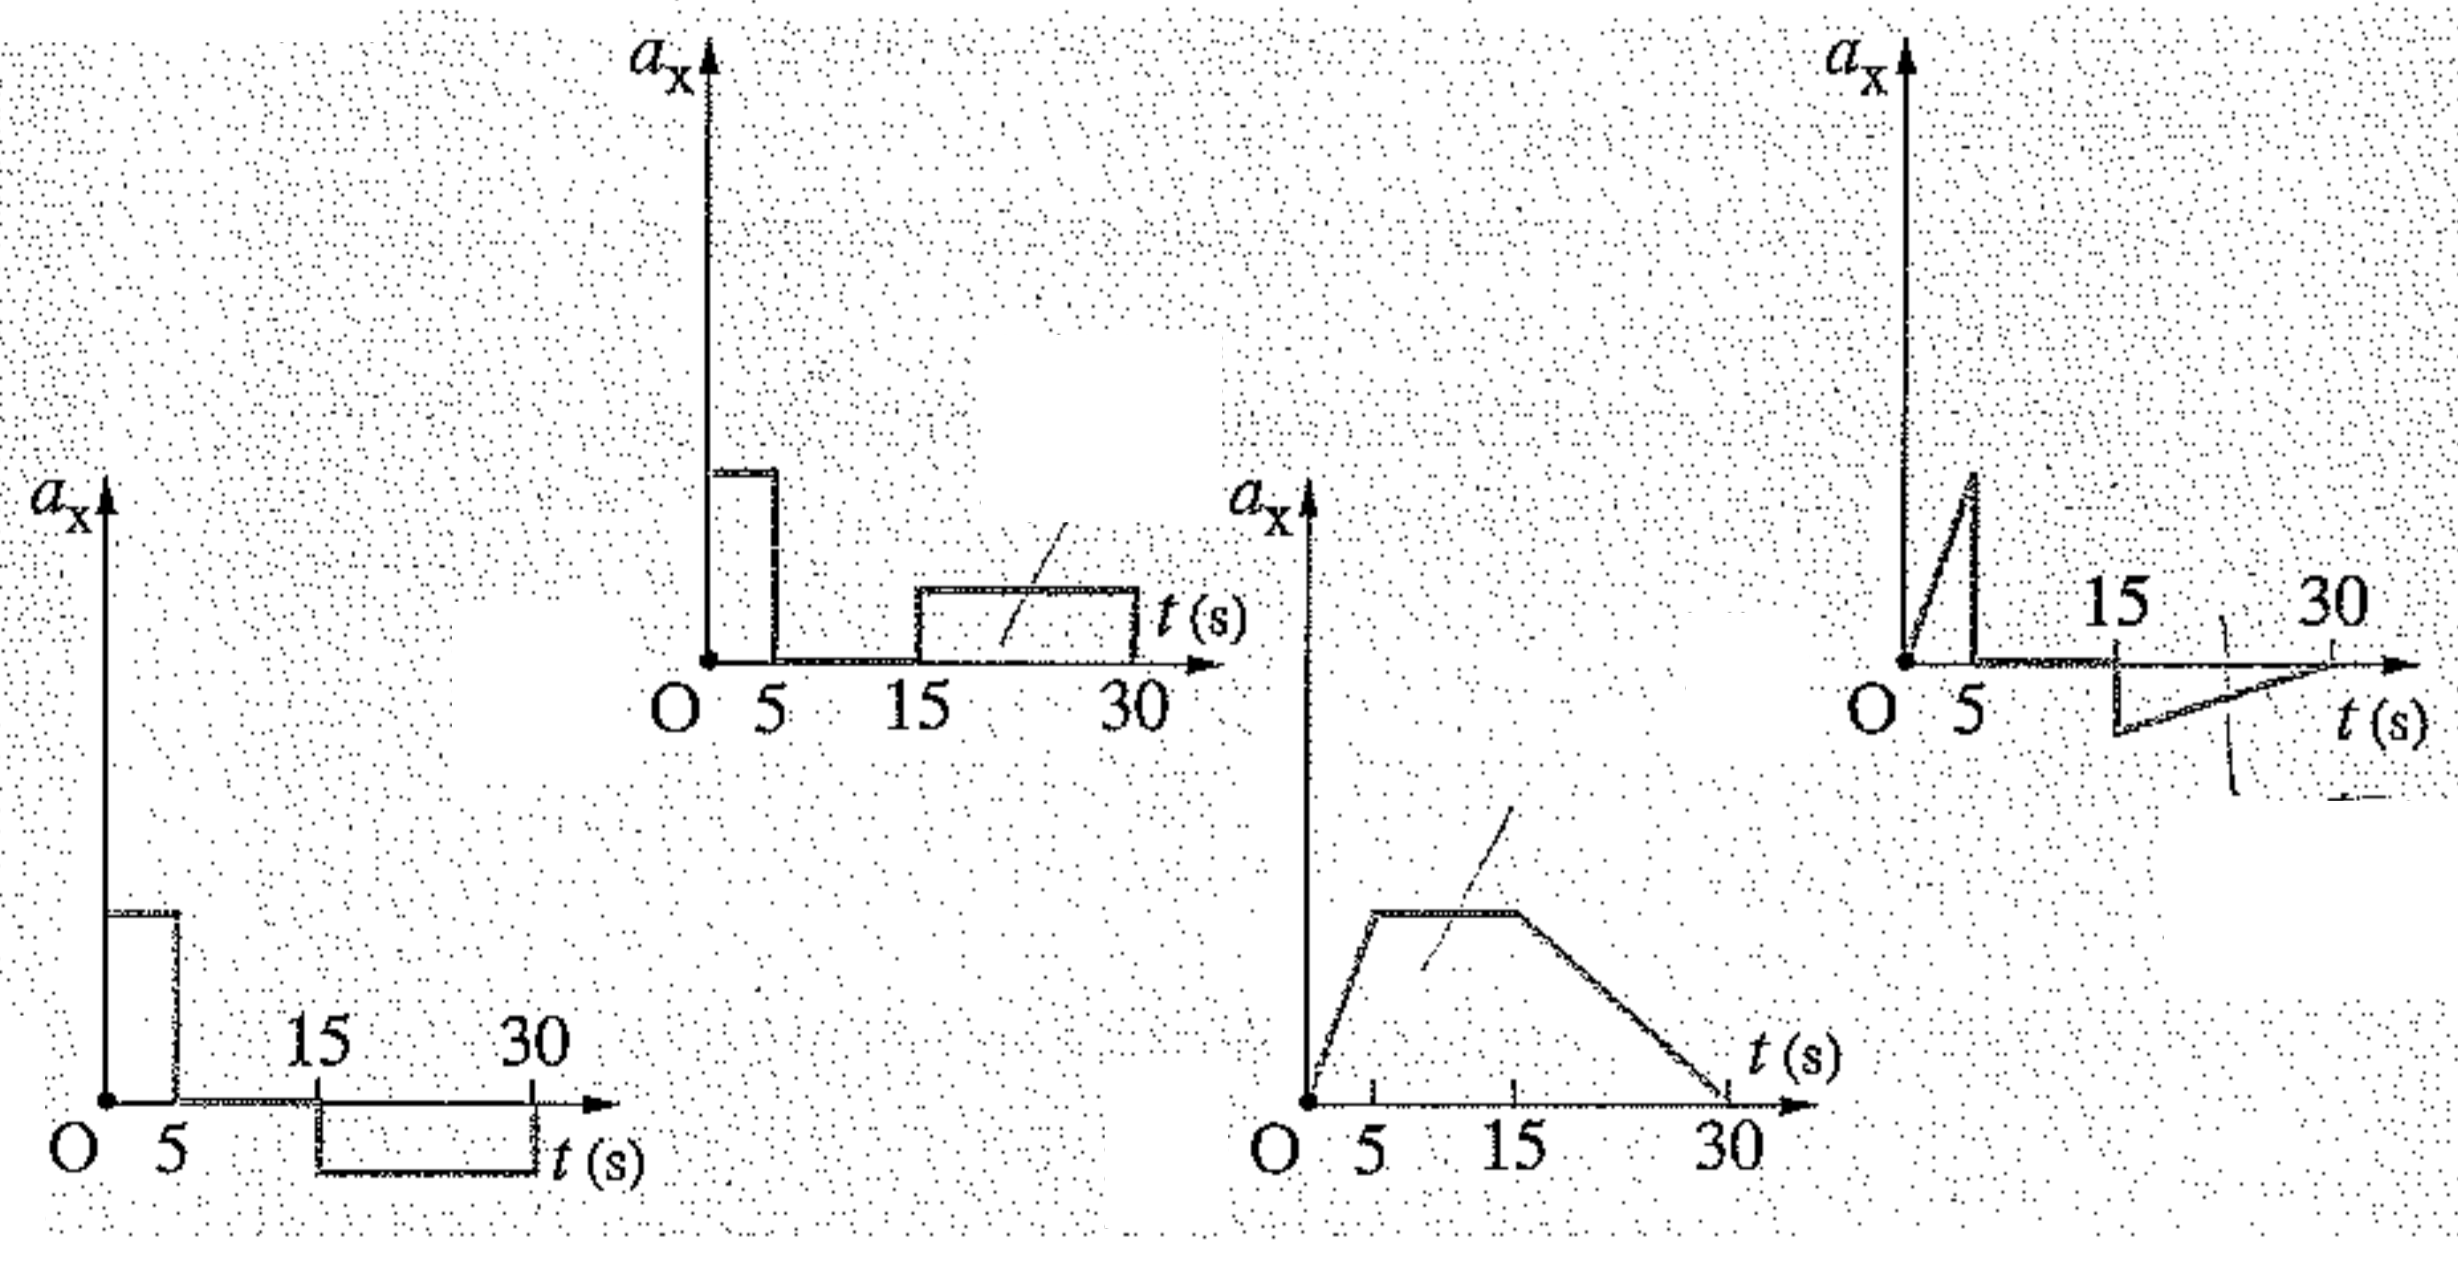
\includegraphics[width=0.93\textwidth]{snelheidsverloop_2}
%\end{flushright}
%\end{figure}
%\end{enumerate}
%
%
%\newpage

% Verticale worp




\end{exercise}

\begin{exercise} Een appel valt van een boom. Zijn valtijd bedraagt $0,5\rm\,s$. Hoe hoog hing de appel?



\end{exercise}

\begin{exercise} Vanaf welke hoogte moet een lichaam vrij vallen om met een snelheid van $100\rm\,m/s$ de grond te bereiken?



\end{exercise}

\begin{exercise} Op het dak van een flatgebouw wordt een bal verticaal
opwaarts geworpen met een snelheid van $10\rm\,m/s$. $4,0\rm\,s$
later bereikt de bal de grond.
\begin{enumerate}
\item Hoe hoog vloog de bal?
\item Hoe hoog is het flatgebouw?
\end{enumerate}

\end{exercise}

\begin{exercise} Een luchtballon stijgt met een snelheid van $8,0\rm\,m/s$. Op
$100\rm\,m$ hoogte laat men een zakje zand vallen. Hoeveel tijd
heeft het zakje nodig om de grond te bereiken?

\end{exercise}

\begin{exercise} Uit een luchtballon laten we een steen vrij vallen. E\'en
seconde later werpen we vanuit hetzelfde punt een tweede steen naar
beneden. Wat is de kleinste beginsnelheid die we de tweede steen
moeten geven opdat ze de eerste nog zou kunnen
inhalen?~\footnote{Druk je antwoord uit als functie van de hoogte
$x$. antw.
$v_0=\frac{x-\frac{1}{2}g(\frac{2x}{g}-t_0)^2}{\frac{2x}{g}-t_0}$}

\end{exercise}

\begin{exercise} Van de boord van een schip valt een loden bol in het water. De
\mbox{boord} bevindt zich $4,0\rm\,m$ boven het wateroppervlak. De
loden bol zinkt vervolgens met de snelheid waarmee hij het water
raakte. Er zijn $6,0\rm\,s$ tussen het tijdstip waarop de bol valt
en ze de bodem van het water bereikt.
\begin{enumerate}
\item Hoe diep is het water?
\item Wat is de gemiddelde snelheid van de bol over het hele
traject?
\end{enumerate}

\end{exercise}

\begin{exercise} Men laat twee lichamen vallen vanuit rust met een tussentijd van
$1\rm\,s$. Hoe lang na de start van het eerste zijn ze $10\rm\,m$
van elkaar verwijderd? \footnote{antw. $1,52\rm\,s$}

\end{exercise}

\begin{exercise} Een open liftkooi stijgt met constante snelheid $10\rm\,m/s$.  Een jongen
die in de kooi staat werpt een bal recht omhoog op het moment dat de
lift $30\rm\,m$ boven de grond is. De beginsnelheid van de bal
t.o.v. de lift is $20\rm\,m/s$. zoek de maximale hoogte die de bal
bereikt en hoe lang het duurt voor de jongen hem terug kan opvangen.
\footnote{antw. $76\rm\,m$; $4,1\rm\,s$}



\end{exercise}

\begin{exercise} Een verticaal vallende steen legt in de laatste seconde, voor hij de grond bereikt, \SI{100}{m} af. Men veronderstelt dat hij vanuit rust vertrok.
\begin{enumerate}
\item Bepaal de snelheid op het ogenblik dat hij de grond bereikt.
\item Bepaal de hoogte vanwaar de steen viel en de tijd die hij daarvoor nodig had.
\end{enumerate}
\begin{oplossing}
\footnote{$v=\frac{x_2-x_1}{t_2-t_1}+\frac{1}{2}g(t_2-t_1)=\frac{\Delta x}{\Delta t}+\frac{1}{2}g\Delta t$
\newline
$t_2=\frac{v_2}{g}=\frac{\Delta t}{2}+\frac{\Delta x}{g\Delta t}$, $x=\frac{1}{2}gt^2=\frac{1}{2g}\left(\frac{\Delta x}{\Delta t}\right)^2+\frac{\Delta x}{2}+\frac{g(\Delta t)^2}{8}$}
\item[\textit{gegeven}]$\Delta t=\SI{1,0}{s}$; $\Delta x=\SI{100}{m}$; $v_0=0$
\item[\textit{gevraagd}]$v_2$, $x_2$, $t_2$
\item[\textit{oplossing}]
\begin{enumerate}
\item 
\begin{minipage}[t]{.7\textwidth}
We kiezen de $x$-as naar beneden zodat de versnelling de valversnelling is, $a=g$. Als we $x_1$ beschouwen als de beginpositie van de beweging die de steen uitvoert in de laatste honderd meter, kunnen we de snelheid vinden waarmee de steen hieraan begint.
\begin{eqnarray*}
&&\Delta x=v_1\Delta t+\frac{1}{2}g\Delta t^2\\
&\Leftrightarrow&v_1=\frac{\Delta x-\frac{1}{2}g\Delta t^2}{\Delta t}
\end{eqnarray*}
\end{minipage}
\begin{minipage}[t][4.5cm][b]{.3\textwidth}
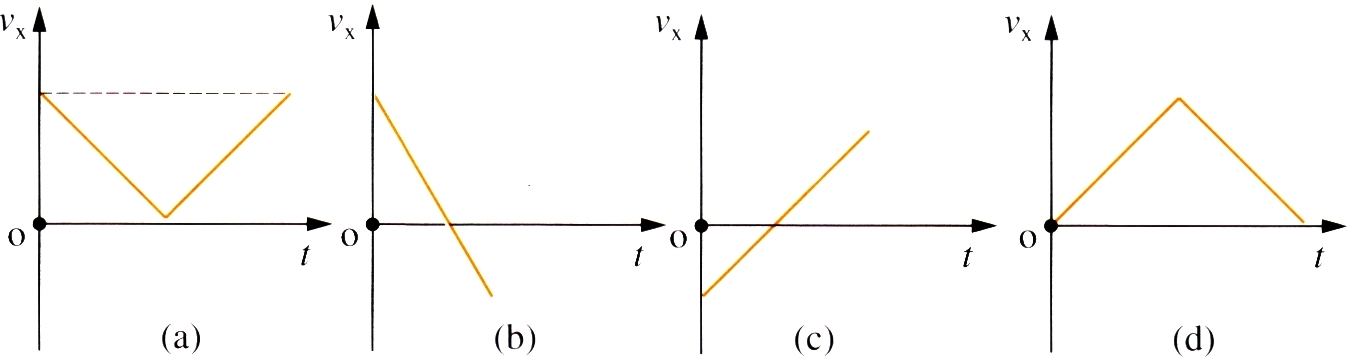
\includegraphics[height=6cm]{valbeweging}
\end{minipage}
\newline
\newline
\newline
Met de formule voor de snelheid van een EVRB, vinden we de snelheid op het einde van het interval.
\begin{eqnarray*}
v_2&=&v_1+g\Delta t\\
&=&\frac{\Delta x-\frac{1}{2}g\Delta t^2}{\Delta t}+g\Delta t\\
&=&\cdots\\
&=&\overline{v}+g\frac{\Delta t}{2}\\
&=&\SI{105}{s}
\end{eqnarray*}
Je kan dit ook afleiden door gebruik te maken van de formule voor gemiddelde snelheid, $\overline{v}=\frac{v_1+v_2}{2}$.
\item Omdat we de snelheid kennen, kunnen we de tijd vinden die de steen nodig heeft gehad om aan deze snelheid te komen. Vervolgens vinden we dan ook de afstand.
\begin{eqnarray*}
t_2=\frac{v_2}{g}=\frac{\overline{v}}{g}+\frac{\Delta t}{2}=\SI{10,7}{s}\\
x_2=\frac{1}{2}gt_2^2=\SI{561}{m}
\end{eqnarray*}
\end{enumerate}
\end{oplossing}



\end{exercise}

\begin{exercise} Men laat een steentje in een put vallen. Na $10\rm\,s$ hoort
men het de bodem bereiken. Men verwaarloost de tijd die het geluid
nodig heeft om de rand van de put te bereiken.
\begin{enumerate}
\item
\begin{enumerate}
\item Bepaal de snelheid van het deeltje na $5,0\rm\,s$ en na $10\rm\,s$
\item Stel de snelheid grafisch voor in functie van de tijd.
\end{enumerate}
\item
\begin{enumerate}
\item Welk deel van de weg heeft het steentje reeds afgelegd na
$5,0\rm\,s$? Hoe diep is de put?
\item Stel de afgelegde weg grafisch voor als functie van de tijd.
\end{enumerate}
\item Was het in het gegeven toegelaten te onderstellen dat de tijd,
die het geluid nodig heeft om de rand van de put te bereiken, te
verwaarlozen is? De snelheid van het geluid is $343\rm\,m/s$.
\end{enumerate}

\end{exercise}

\begin{exercise} Iemand gooit vanaf de rand van een klif een steen omhoog met
een snelheid van $10\rm\,m/s$. Na 7 seconden hoort hij de steen in
de oceaan vallen. Hoe hoog is het klif? De snelheid van het geluid
is $343\rm\,m/s$.

\end{exercise}

\begin{exercise} Iemand aan de rand van een klif laat een steen vallen en hoort
$3,3\rm\,s$ later het geluid waarmee de steen in de oceaan plonst.
De snelheid van het geluid is $343\rm\,m/s$. Hoe hoog is het
klif?~\footnote{$x_0=v_2t_2+\frac{v_2^2}{g}+v_2\sqrt{(t_2g+v_2)^2-t_2^2}$}


\end{exercise}

\begin{exercise} Schets het $x(t)$- $v(t)$- en $a(t)$-diagram bij een EVRB met $x_0=2,0\rm\,m$, $v_0=20\rm\,m/s$ en $a=-2,0\rm\,m/s^2$.

\end{exercise}

\begin{exercise} Hieronder worden vier rechtlijnige bewegingen voorgesteld in een grafiek. Dan is de afgelegde weg na $6~\rm s$ het grootst in figuur:
\begin{figure}[h]
\begin{center}
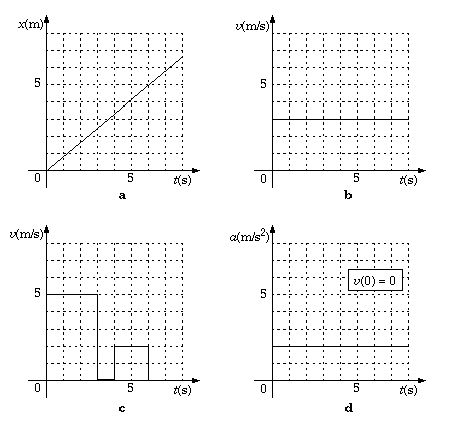
\includegraphics[width=0.8\textwidth, angle=0]{4erbs}
\end{center}
\end{figure}
\footnote{antw. d}


\end{exercise}

\begin{exercise} De snelheidsfunctie van een auto wordt voorgesteld op de figuur. 
\begin{figure}[h]
\centering
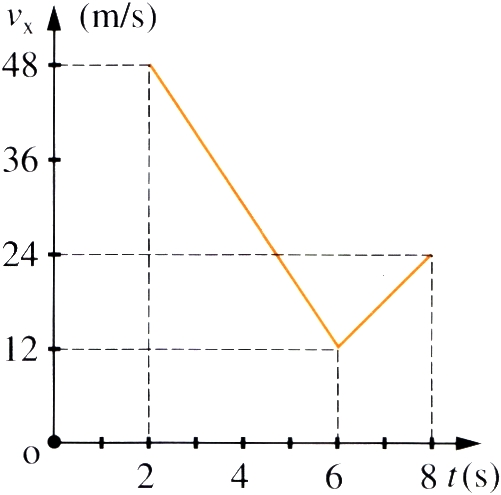
\includegraphics[width=0.32\textwidth]{racewagen}
\end{figure}
\newline
Beantwoord de volgende vragen.
\begin{enumerate}
\item Beschrijf de beweging. 
\item Bereken de positieverandering tussen de tweede en de achtste seconde. 
\item Bereken de gemiddelde snelheid tussen de tweede en de achtste seconde. 
\item Bereken de gemiddelde versnelling. 
\item Teken in de grafiek het snelheidsverloop van een auto die met deze gemiddelde versnelling
zou rijden en op $t=2\rm\,s$ zou beginnen met dezelfde beginsnelheid als de auto in de opgave.
\end{enumerate}



\end{exercise}

\begin{exercise} In de onderstaande figuur is de positie $x$ van Tieme tijdens een fietstocht
gegeven als functie van de tijd $t$.
\begin{figure}[h]
\begin{center}
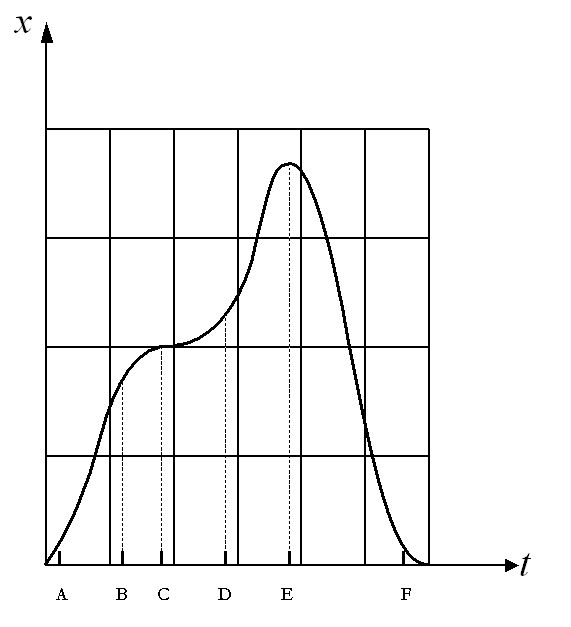
\includegraphics[width=0.4\textwidth, angle=0]{versnelling_xtgrafiek}
\end{center}
\end{figure}
\newline
Welke uitspraak is correct? Op de volgende tijdstippen heeft Tieme
een versnelling die positief is:
\begin{enumerate}
\item C en E
\item B, D en E
\item A, D en F
\item A en D
\end{enumerate}
\footnote{antwoord c}

\end{exercise}

\begin{exercise} Onderstaande grafiek geeft het
tijdsverloop aan van de positie $x$ van een wagen die met een
constante versnelling vanuit rust vertrekt. Op de verticale as kan
men $x$ aflezen, op de horizontale $t^2$.
\begin{figure}[h]
\begin{center}
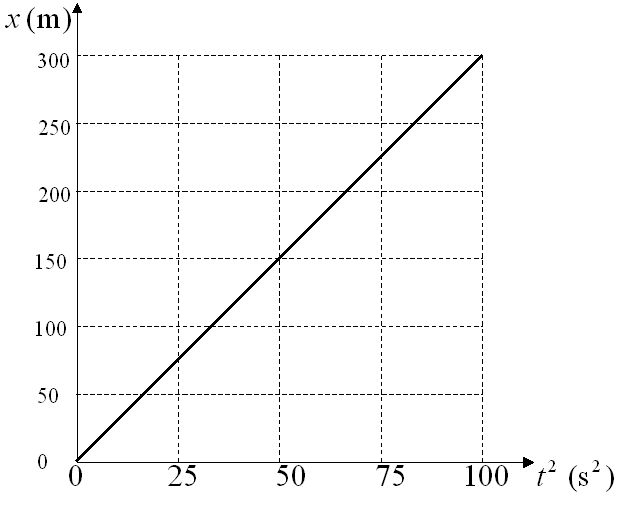
\includegraphics[width=0.4\textwidth]{grafiek_xt}
\end{center}
\end{figure}
\newline
De grootte van de versnelling van de wagen is dan:
\begin{enumerate}
\item 2 m/s$^2$
\item 3 m/s$^2$
\item 6 m/s$^2$
\item 12 m/s$^2$
\end{enumerate}



\end{exercise}

\begin{exercise} Een bolvormig voorwerp valt verticaal in lucht vanaf een grote
hoogte. De luchtweerstand is \textit{niet} te verwaarlozen. De
beweging wordt het best weergegeven door de figuur:
\begin{figure}[h]
\begin{center}
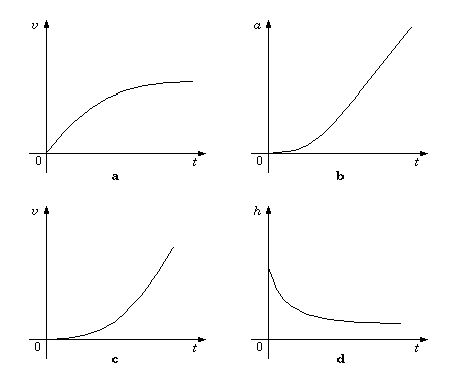
\includegraphics[width=0.8\textwidth, angle=0]{vallend_voorwerp_wrijving}
\end{center}
\end{figure}
\footnote{Antwoord (a) is juist.}

\begin{oplossing}
\item De snelheid waarmee de patrouilleleider vooruit gaat, is de snelheid waarmee de $x$-co\"ordinaat verandert. De snelheid waarmee het mandje omhoog gaat, is gelijk aan de de snelheid waarmee de lengte $l$ langer wordt. Dus
\begin{eqnarray*}
v&=&\frac{dx}{dt}\\
v'&=&\frac{dl}{dt}.
\end{eqnarray*}
Nu zijn de lengte $l$ en de positie $x$ aan elkaar gerelateerd via de stelling van Pythagoras, $l^2=x^2+h^2$. De lengte $l$ is dus te schrijven in functie van $x$: $l=\sqrt{x^2+h^2}$. Nu zijn zowel $l$ als $x$ functies van $t$ en kunnen we $l(t)$ als een samengestelde functie beschouwen:
\begin{eqnarray*}
l(t)=\sqrt{\left(x(t)\right)^2+h^2}
\end{eqnarray*}
Wanneer we $l$ willen afleiden, moeten we dus de kettingregel\footnote{Merk op dat we hier met drie samenstellende functies te maken hebben. Eerst wordt $t$ afgebeeld op $x(t)$, vervolgens wordt $x$ afgebeeld op $x^2+h^2$ en de laatste functie in de schakel is de wortelfunctie.} gebruiken.
\begin{eqnarray*}
\frac{dl}{dt}&=&\frac{dl}{dx}\frac{dx}{dt}\\
&=&\frac{2x}{2\sqrt{x^2+h^2}}\frac{dx}{dt}\\
&=&\frac{x}{\sqrt{x^2+h^2}}v
\end{eqnarray*}
De uitspraak met de vectoren is fout omdat de snelheden een verschillende richting hebben
\end{oplossing}

\end{exercise}















\end{document}
